\documentclass[10pt]{article}

\usepackage{lmodern}
\usepackage{amsmath,amssymb,amsthm}
\usepackage{bm}
\usepackage{booktabs}
\usepackage{multirow}
\usepackage{array}
\usepackage{graphicx}
\usepackage{xcolor}
\usepackage{algorithm}
\usepackage{algpseudocode}
\usepackage{microtype}
\usepackage{cite}
\usepackage{enumitem}
\usepackage{fancyhdr}
\usepackage[top=0.66in,bottom=0.66in,left=0.80in,right=0.80in]{geometry}
\usepackage[colorlinks=true,linkcolor=blue!55!black,citecolor=blue!55!black,urlcolor=blue!55!black]{hyperref}

\linespread{1.05}
\renewcommand{\arraystretch}{1.2}
\newcommand{\tblfont}{\fontsize{8.5pt}{10.4pt}\selectfont}
\setlength{\intextsep}{5pt plus 2pt minus 2pt}
\setlength{\textfloatsep}{7pt plus 2pt minus 2pt}
\setlength{\abovecaptionskip}{3.5pt}
\setlength{\belowcaptionskip}{1.5pt}
\setlength{\emergencystretch}{2em}

\newtheorem{theorem}{Theorem}
\pagestyle{fancy}
\fancyhf{}
\renewcommand{\headrulewidth}{0.4pt}
\fancyhead[L]{\footnotesize \textit{DTRA: Dynamic Topology Ring Architecture}}
\fancyhead[R]{\footnotesize \textit{Continual Visuomotor Control ($K=100$)}}
\fancyfoot[C]{\thepage}

\title{\vspace{-2.3em}\rule{\linewidth}{2pt}\\[0.32em]\textbf{DTRA: Dynamic Topology Ring Architecture for Zero-Forgetting Continual Visuomotor Control via Hyperspherical Topological Isolation}\\[0.25em]\rule{\linewidth}{0.8pt}\vspace{-0.85em}}

\author{
  \textbf{Seungjoon Son}\\
  Independent AI \& Robotics Researcher, Daejeon, Republic of Korea\\
  Repository: \url{https://github.com/5Color/dtra}\\
  Predecessor: \url{https://github.com/5Color/abk-vla}
}
\date{November 2026}

\begin{document}
\maketitle

\begin{center}\vspace{-0.4em}
\begin{minipage}{0.92\linewidth}
\centering
\textit{``Scaling up parameters just to remember a hundred chores? How adorable.\\ Geometry does it with twenty-seven.''} --- \textsc{Seungjoon Son}
\end{minipage}
\end{center}
\vspace{0.1em}

\begin{abstract}
Prevailing robot learning paradigms assume all sensorimotor skills must be unified within a single, homogeneous parameter space optimized end-to-end from scratch. In lifelong continual learning, this structural uniformity forces new experiences to overwrite prior motor memories unless mitigated by massive replay buffers or billion-parameter scale. We present \textbf{DTRA} (\emph{Dynamic Topology Ring Architecture}), a geometry- and topology-first framework for replay-free, Task-ID-free continual visuomotor control. Building on our predecessor ABK-VLA~\cite{son2026abkvla} (Zenodo DOI: \texttt{10.5281/zenodo.24208545})---which established $C^2$-continuous Clamped Cubic B-Spline action compression and cosine prototype routing at $K=4$ tasks---DTRA models motor skills as isolated elliptical hypertube rings on the unit hypersphere $\mathbb{S}^{63}$ and resolves the high-density bottlenecks exposed when scaling to $K=100$ sequential 7-DoF LIBERO manipulation tasks (\texttt{libero\_10 + libero\_90}). Specifically, we introduce four complementary mechanisms: (i) a \textbf{No-Encroachment Constraint} that caches each prior task's raw query anchor $\mu_j$ and self-similarity floor $s_{jj}$ to prevent newly registered keys from invading prior Voronoi cells, (ii) \textbf{Two-Stage Top-$M$ Common-Mode Cancellation} that strips shared scene background and duplicate-instruction modes before fine spatial-proprioceptive reranking, (iii) \textbf{Two-Timescale Snap-Back} separating chunk-end elastic reset (\texttt{chunk\_snap\_back()}, $\Delta\mathbf{z}_i \leftarrow \mathbf{0}$) from episode-end refractory reset (\texttt{episode\_snap\_back()}, $0.0000$ drift norm), and (iv) \textbf{SharedBasisBank} factorizing knot-space ($N_k=6$) motor primitives with strict optimizer exclusion ($\nabla_\theta=0$, zero \texttt{AdamW} silent drift). Across 3-seed 8-task 3D Meta-World ablations, DTRA preserves \textbf{0.0\% forgetting} and \textbf{100.0\% multimodal routing} with constant $O(1)$ active execution ($1.87\,$ms from $K=1 \to 8$) and \textbf{51.4\% severe OOD SR} (vs.\ $23.6\%$ for Frozen MLP and $2.2\%$ for ABK DoG). Scaled to \textbf{LIBERO-100} ($K=100$) under strict encoder parity (3-seed \texttt{\_locked.json} Mean $\pm$ Std across Seeds~[42, 100, 2026]), DTRA achieves \textbf{87.00 $\pm$ 0.86\% Final Mean SR} (peak 87.80\% on Seed~42; vs.\ 70.33 $\pm$ 1.18\% Frozen MLP baseline, \textbf{+16.67\%p}), preserves \textbf{99.90 $\pm$ 0.13\% overall} and \textbf{99.68 $\pm$ 0.45\% duplicate-instruction routing} (vs.\ 41.76 $\pm$ 2.09\% baseline crash, \textbf{+57.93\%p}), maintains positive backward transfer (+0.20 $\pm$ 0.72\% BWT, $0.0000$ snap drift), and compresses 100 tasks into \textbf{27 shared primitive bases (73\% basis reduction)}. These results demonstrate replay-free, Task-ID-free control across a single VLM-free 100-task continual stream, with improved final success and duplicate-instruction routing relative to the evaluated Frozen MLP baseline under matched-encoder conditions.
\end{abstract}

% ==========================================================================
\section{Introduction}
\label{sec:intro}
% ==========================================================================

\textbf{Rejection of Monolithic Parameter Interference \& Topological Scalability.}
Prevailing Vision-Language-Action (VLA) paradigms~\cite{vaswani2017attention,brohan2023rt1,brohan2023rt2,kim2024openvla,black2024pi0} pack sensorimotor skills into monolithic dense parameter spaces optimized end-to-end. In lifelong continual learning~\cite{wolczyk2021continual,liu2023libero}, shared matrix updates for task $T_k$ systematically disrupt prior motor circuits $T_0, \dots, T_{k-1}$. Biological intelligence instead stabilizes myelinated circuits ($\nabla_\theta = 0$) while attaching modular loops: when continuous trajectories are encoded smoothly on $\mathbb{S}^{63}$ and partitioned geometrically, lifelong retention stems from topological isolation using $27$ frozen bases and zero rehearsal rather than billion-parameter bloat.

\begin{figure}[ht!]
  \centering
  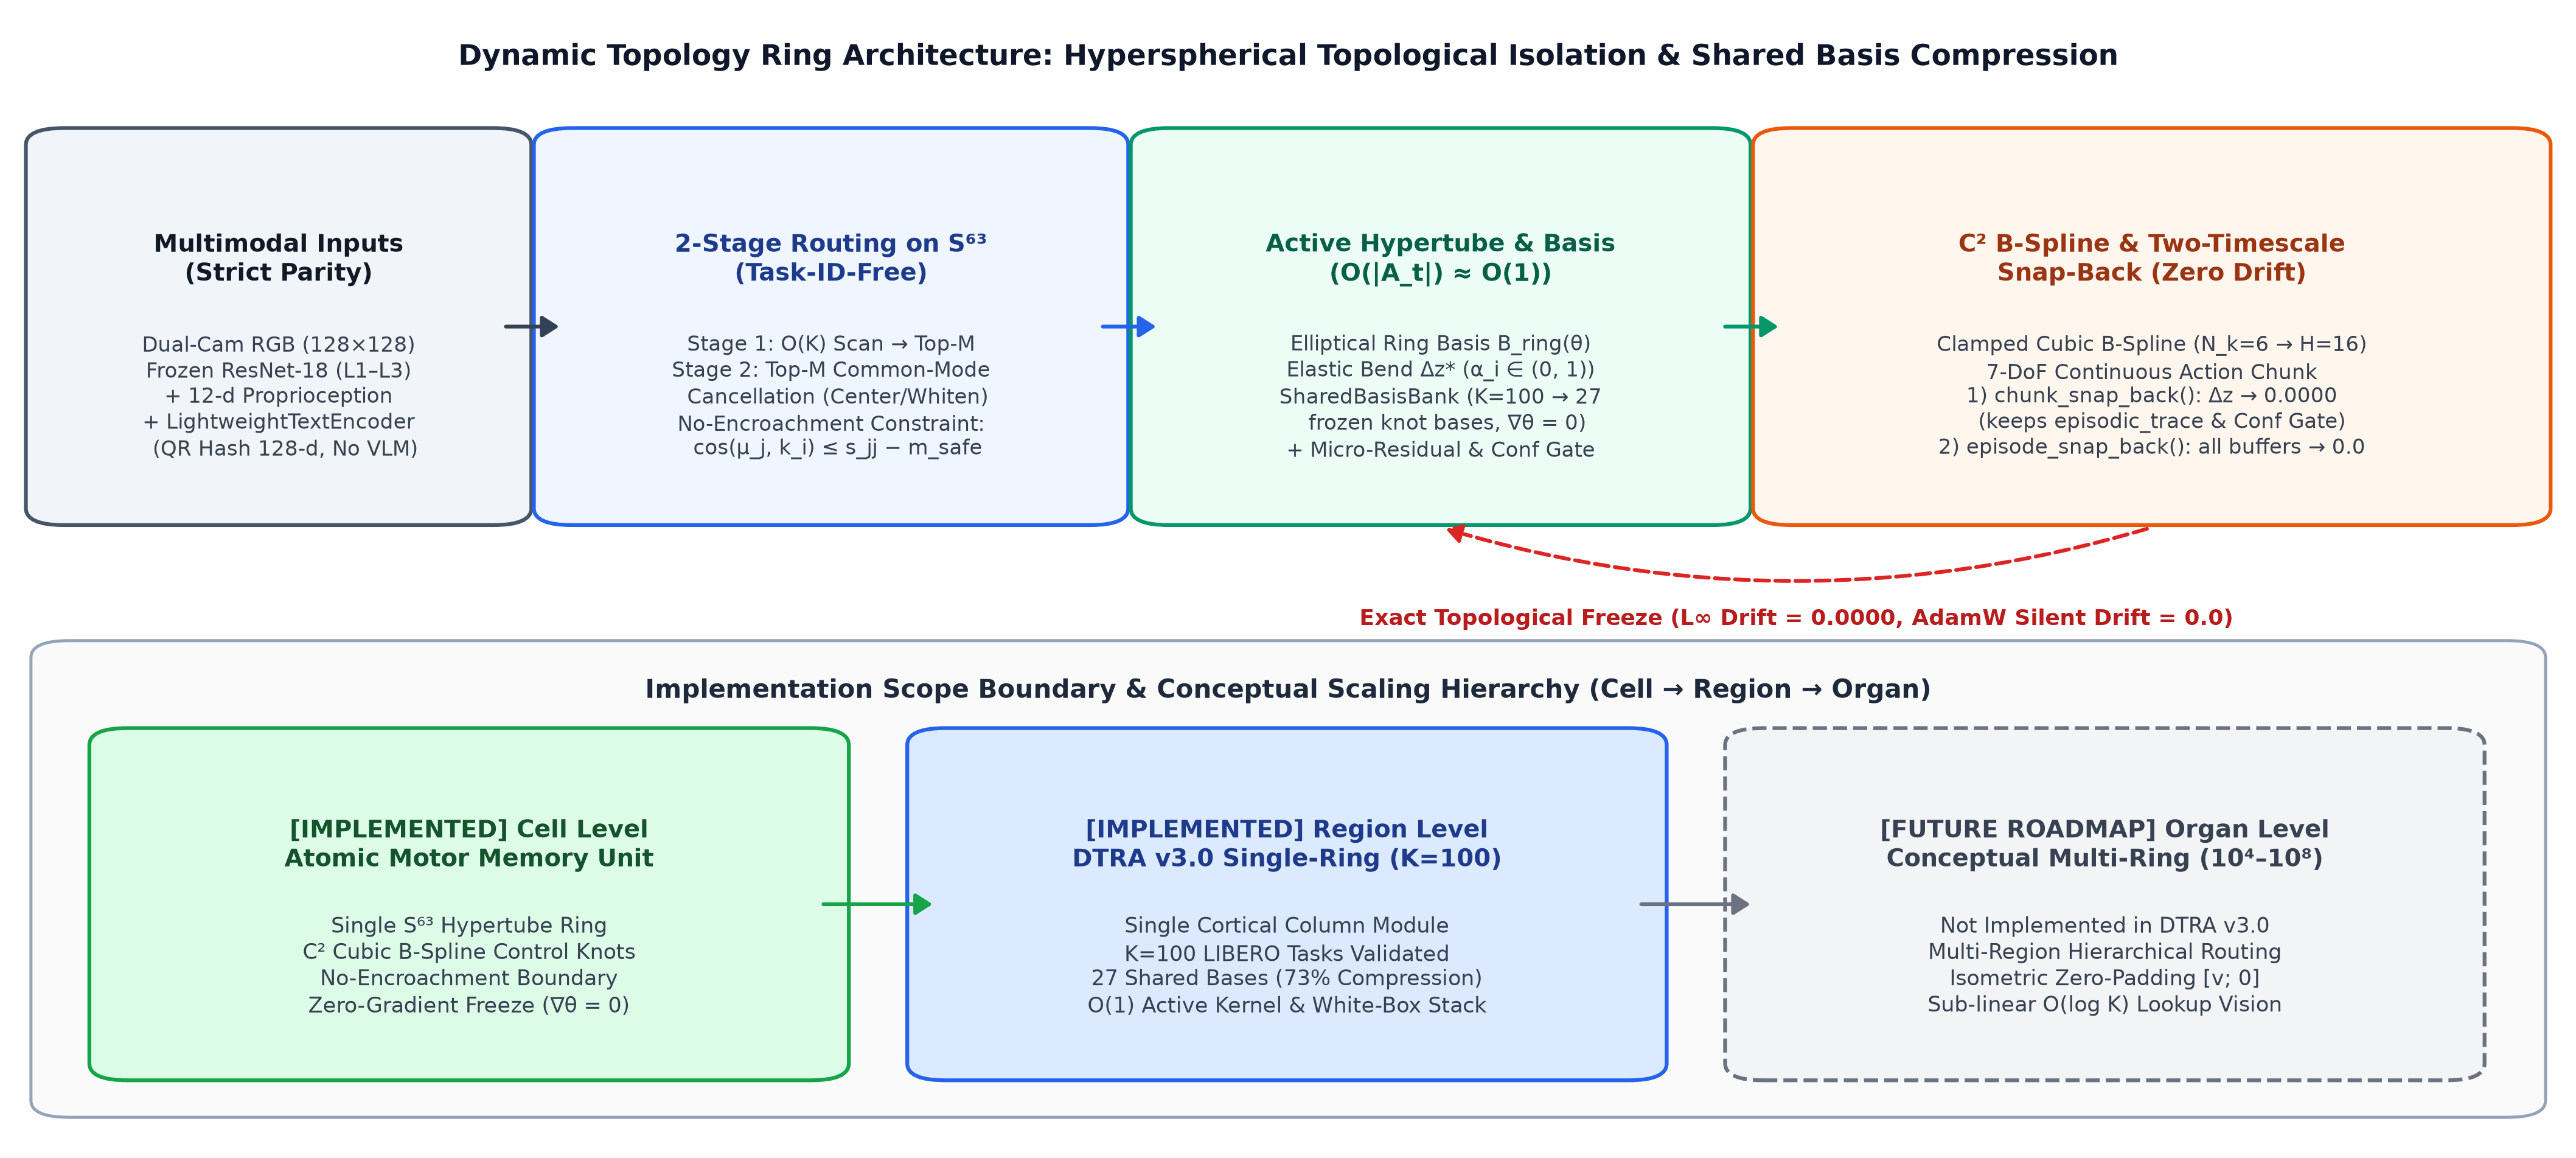
\includegraphics[width=0.71\textwidth]{../../outputs/figures/fig6_dtra_v3_architecture_schematic.png}
  \caption{\textbf{DTRA end-to-end architecture and implementation scope boundary.} \textbf{Top:} Strict-parity multimodal perception (\texttt{Frozen ResNet-18} + proprioception + \texttt{LightweightTextEncoder}), two-stage Top-$M$ common-mode cancellation with No-Encroachment keys on $\mathbb{S}^{63}$, active hypertube + \texttt{SharedBasisBank} ($K=100 \to 27$ frozen bases), $C^2$ cubic B-Spline decoding, and Two-Timescale Snap-Back ($L_\infty$ drift $= 0.0000$). \textbf{Bottom:} Explicit scope separation between the implemented \emph{Cell} / single-ring \emph{Region} ($K=100$) modules validated in this paper and the conceptual \emph{Organ} ($10^4$--$10^8$ tasks) future work roadmap.}
  \label{fig:dtra_v3_arch}
\end{figure}

\textbf{Research Lineage: ABK-VLA ($K=4$) $\to$ DTRA ($K=100$).}
Our prior work \textbf{ABK-VLA}~\cite{son2026abkvla} (DOI: \texttt{10.5281/zenodo.24208545}) compressed $H=16$ chunks into $N_k=6$ clamped cubic B-Spline knots ($C^2$-continuous), reaching $99.98\%$ routing across $K=4$ tasks. Extending it to 8-task Meta-World resolved $O(K)$ chaining latency and DoG visual fragility via $\mathbb{S}^{63}$ hypertubes at $K=8$.

However, scaling twenty-fold further to \textbf{LIBERO-100} ($K=100$ dual-camera tasks) exposes two harsh high-density bottlenecks:
\begin{enumerate}[leftmargin=*,itemsep=1.5pt,topsep=2pt]
  \item \textbf{Voronoi Encroachment Under Duplicate/Near-Duplicate Language (\texttt{Dup-Lang}):} LIBERO-100 contains $30$ tasks across $13$ identical-instruction groups in shared scenes. Unconstrained key repulsion pushes new keys $\mathbf{k}_i$ into prior Voronoi cells $\mathbf{k}_j$ ($j < i$), collapsing baseline \texttt{Dup-Lang} routing from $100.0\%$ ($K=10$) to 41.76 $\pm$ 2.09\% ($K=100$).
  \item \textbf{Linear $O(K)$ Head Growth vs.\ Expressivity:} Independent per-task heads grow linearly to $100$ blocks ($151.67\,$MB), whereas naive weight sharing causes severe backward interference.
\end{enumerate}

\textbf{Core Contributions (Region Scope).}
DTRA resolves both bottlenecks under strict encoder parity:
\begin{itemize}[leftmargin=*,itemsep=1.5pt,topsep=2pt]
  \item \textbf{No-Encroachment Margin Refinement:} Caches prior anchors $\mu_j$ and self-similarity floors $s_{jj} = \cos(\mu_j, \mathbf{k}_j)$, projecting out repulsive updates that steal Voronoi territory from prior tasks $0 \dots i-1$.
  \item \textbf{Two-Stage Top-$M$ Common-Mode Cancellation (CMC):} Retrieves Top-$M$ ($M=5$) candidates via $O(K)$ cosine scan, then strips shared language/scene modes to amplify DualCam grids ($4\times 4 / 2\times 2$ + DoG) and proprioception, lifting $K=100$ \texttt{Dup-Lang} routing from 41.76 $\pm$ 2.09\% to \textbf{99.68 $\pm$ 0.45\%}.
  \item \textbf{\texttt{SharedBasisBank} + Zero \texttt{AdamW} Silent Drift:} Compresses $100$ tasks into \textbf{27 shared knot bases (73\% reduction)} while excluding frozen bases from \texttt{AdamW} (\texttt{requires\_grad=False}, $L_\infty$ silent drift $= 0.0$).
  \item \textbf{Two-Timescale Snap-Back:} Resets $\Delta\mathbf{z}_i \leftarrow \mathbf{0}$ after each chunk (\texttt{chunk\_snap\_back()}) while retaining \texttt{episodic\_trace} + \texttt{Conf Gate}, followed by full reset (\texttt{episode\_}\allowbreak\texttt{snap\_back()} $\to 0.0000$).
  \item \textbf{LIBERO-100 Continual Control under Strict Encoder Parity:} Establishes \textbf{87.80\%} (Seed~42; \textbf{87.00 $\pm$ 0.86\%} over observed seeds) Final Mean SR for replay-free, Task-ID-free LIBERO-100 control with 27 frozen bases.
\end{itemize}

\clearpage
% ==========================================================================
\section{Related Work}
\label{sec:related}
% ==========================================================================

\subsection{Continual Learning and Parameter Isolation}
Continual learning algorithms negotiate the stability--plasticity dilemma~\cite{mccloskey1989catastrophic,french1999catastrophic,parisi2019continual}. Regularization methods such as Elastic Weight Consolidation (EWC)~\cite{kirkpatrick2017ewc}, Synaptic Intelligence (SI)~\cite{zenke2017si}, Memory Aware Synapses (MAS)~\cite{aljundi2018mas}, and Riemannian Walk~\cite{chaudhry2018rwalk} penalize quadratic drift around prior optima, yet still fail when sequential gradients overwrite sensitive low-level visuomotor pathways. Rehearsal methods such as GEM~\cite{lopezpaz2017gem}, A-GEM~\cite{chaudhry2019agem}, Experience Replay (CLEAR)~\cite{rolnick2019clear}, and Dark Experience Replay~\cite{buzzega2020der} buffer historical demonstrations, sacrificing pure replay-free autonomy and struggling when buffer capacity saturates at $K=100$.

Parameter-isolation architectures---including Progressive Neural Networks~\cite{rusu2016pnn}, PackNet~\cite{mallya2018packnet}, and Hard Attention to the Task~\cite{serra2018hat}---prevent gradient interference structurally, yet either require ground-truth test-time Task-IDs or scale linearly in active forward compute. Prompt-pool approaches such as L2P~\cite{wang2022l2p}, DualPrompt~\cite{wang2022dualprompt}, and CODA-Prompt~\cite{smith2023coda} route frozen vision backbones without Task-IDs, but remain confined primarily to discrete classification rather than $C^2$-smooth continuous 7-DoF trajectory synthesis. Table~\ref{tab:paradigm_compare} contrasts these paradigms structurally against DTRA.


\begin{table}[t]
  \centering
  \caption{Structural comparison of continual visuomotor control paradigms. DTRA unifies Task-ID-free inference, zero rehearsal memory, exact parameter freezing ($\nabla_\theta = 0$), constant $O(1)$ active kernel execution, and sub-linear basis sharing within a white-box hyperspherical routing stack.}
  \label{tab:paradigm_compare}
  \tblfont
  \setlength{\tabcolsep}{3.0pt}
  \begin{tabular}{lccccccc}
    \toprule
    \textbf{Paradigm / Method} & \textbf{Task-Free} & \textbf{Replay-Free} & \textbf{$\nabla_\theta=0$} & \textbf{Active} & \textbf{Bases / Scaling} & \textbf{Dup-Lang} & \textbf{VLM-Free} \\
    \midrule
    Naive Fine-Tuning & \checkmark & \checkmark & $\times$ & $O(1)$ & Monolith & $\times$ & \checkmark \\
    EWC / RWalk~\cite{kirkpatrick2017ewc,chaudhry2018rwalk} & \checkmark & \checkmark & $\times$ & $O(1)$ & Monolith+Pen. & $\times$ & \checkmark \\
    GEM / ER (5\%)~\cite{lopezpaz2017gem,rolnick2019clear} & \checkmark & $\times$ & $\times$ & $O(1)$+Buf & Monolith & $\times$ & \checkmark \\
    PNN / PackNet~\cite{rusu2016pnn,mallya2018packnet} & $\times$ & \checkmark & Masked & $O(K)$ & Linear $O(K)$ & N/A & \checkmark \\
    L2P / CODA-Prompt~\cite{wang2022l2p,smith2023coda} & \checkmark & \checkmark & Backb. & Pool & Prompts & Partial & ViT \\
    SeqLoRA / KeepLoRA~\cite{parsa2026seqlora,luo2026keeplora} & Depends & Mostly & Adapter & $O(\text{rank})$ & LoRA & $\times$ & Diff/VLM \\
    OrthoSkillVLA~\cite{wang2026orthoskill} & $\times$ & Partial & Subsp. & VLM Fwd & Grad Subsp. & $\times$ & VLM \\
    ABK-VLA v1.1.3~\cite{son2026abkvla} & \checkmark & \checkmark & \checkmark & $O(K)$ & Linear $O(K)$ & $\times$ (DoG) & \checkmark \\
    \textbf{DTRA (Ours)} & \textbf{\checkmark} & \textbf{\checkmark} & \textbf{\checkmark ($0$)} & \textbf{$O(1)$} & \textbf{27 ($-73\%$)} & \textbf{\checkmark (CMC)} & \textbf{\checkmark} \\
    \bottomrule
  \end{tabular}
\end{table}


\subsection{Visuomotor Action Chunking and Continual PEFT Approaches}
Action chunking policies including ACT~\cite{zhao2023act}, Diffusion Policy~\cite{chi2023diffusion}, OpenVLA~\cite{kim2024openvla}, $\pi_0$~\cite{black2024pi0}, and 3D view transformers~\cite{shridhar2022peract,goyal2023rvt} stabilize closed-loop control by predicting temporally extended trajectories, whereas classical movement primitives (DMPs~\cite{ijspeert2013dmp}, ProMP~\cite{paraschos2013promp}) and spline frameworks~\cite{piegl1997nurbs,deboor1978splines} represent motions analytically. Building on ABK-VLA~\cite{son2026abkvla}, DTRA compresses chunks into smooth $C^2$-continuous cubic B-Spline knots.

In continual parameter-efficient fine-tuning (PEFT)~\cite{hu2022lora}, gradient projection memory~\cite{saha2021gpm} and orthogonal LoRA variants such as O-LoRA~\cite{wang2023olora}, InfLoRA~\cite{liang2024inflora}, residual-gradient adaptation in \textbf{KeepLoRA}~\cite{luo2026keeplora} (originally developed for continual VLM and visual classification benchmarks), and diffusion-domain bilevel orthogonal LoRA in \textbf{SeqLoRA}~\cite{parsa2026seqlora} (designed for continual multi-concept text-to-image generation) constrain adapter updates inside shared matrices. Extending orthogonal subspace adaptation directly into robotics, \textbf{OrthoSkillVLA}~\cite{wang2026orthoskill} studies replay-free continual skill adaptation in pretrained VLA models. Its experimental protocol differs from our single VLM-free 100-task continual stream; we therefore discuss it as related work without a direct numerical ranking.

% ==========================================================================
\section{Mathematical Preliminaries}
\label{sec:prelim}
% ==========================================================================

\subsection{Strict-Parity Multimodal Hyperspherical Embedding (\texorpdfstring{$\mathbb{S}^{127} \to \mathbb{S}^{63}$}{S127 -> S63})}
At each control step $t$, all compared parity arms share an identical frozen feature extractor $\mathcal{E}(\cdot)$ combining:
\begin{enumerate}[leftmargin=*,itemsep=1.5pt]
  \item \textbf{Dual-Camera Visual Encoding:} Agent-view and wrist-camera RGB frames pass through a frozen ImageNet-pretrained \texttt{ResNet-18}~\cite{he2016resnet} backbone preserving $4\times 4$ and $2\times 2$ spatial pooling grids alongside Difference-of-Gaussians (DoG) low-pass spatial parity cues ($\mathbf{v}_t \in \mathbb{R}^{d_v}$), plus proprioceptive joint/end-effector states $\mathbf{q}_t$.
  \item \textbf{Deterministic Text Instruction Hashing:} Instructions are encoded deterministically by the \texttt{Lightweight}\allowbreak\texttt{TextEncoder} (unigram/bigram hashing without learned LLM weights) into unit vector $\ell_{\text{task}} \in \mathbb{S}^{d_\ell - 1}$.
\end{enumerate}
Normalized visual-proprioceptive and linguistic vectors form unified query key $\mathbf{x}_t = \mathrm{norm}([\mathbf{v}_t;\, \mathbf{q}_t;\, \ell_{\text{task}}]) \in \mathbb{S}^{127}$ and project into the working topological manifold $\mathbb{S}^{63}$ via orthogonal $P_{\text{topo}} \in \mathbb{R}^{64 \times 128}$:
\begin{equation}
  \mathbf{c}_t = \mathrm{norm}\bigl(P_{\text{topo}} \mathbf{x}_t\bigr) \in \mathbb{S}^{63}, \qquad \|\mathbf{c}_t\|_2 = 1.
\end{equation}

\subsection{Clamped \texorpdfstring{$C^2$}{C2} Cubic B-Spline Action Chunking (\texorpdfstring{$N_k = 6 \to H = 16$}{Nk=6 -> H=16})}
Rather than predicting $H \times d_a$ raw joint/delta actions directly at high-frequency control ticks, DTRA encodes each chunk $\mathbf{A}_t \in \mathbb{R}^{16 \times d_a}$ in the $N_k=6$ control-knot subspace $\mathbf{P} \in \mathbb{R}^{6 \times d_a}$ via a fixed, frozen clamped cubic B-Spline synthesis matrix $\mathbf{B}_{\text{spline}} \in \mathbb{R}^{16 \times 6}$:
\begin{equation}
  \mathbf{A}_t = \mathbf{B}_{\text{spline}} \mathbf{P}_t, \qquad \sum_{n=0}^{5} (\mathbf{B}_{\text{spline}})_{h,n} = 1 \;\; \forall h \in \{0,\dots,15\},
\end{equation}
executing the first \texttt{exec\_steps=8} steps in closed-loop receding horizon before re-querying. This parameterization yields intrinsic low-pass OOD noise immunity while preserving $C^2$ position, velocity, and acceleration continuity across interior knot transitions (proven formally in Appendix~\ref{app:proofs}).

\subsection{Spherical Voronoi Partitioning \& High-Density Collision Failure}
Let $\{\mathbf{k}_j\}_{j=1}^{K} \subset \mathbb{S}^{63}$ denote consolidated routing keys. Standard 1-stage cosine routing assigns $\mathbf{c}_t$ to Voronoi cell $\mathcal{V}_j = \{\mathbf{c} \in \mathbb{S}^{63} : \langle \mathbf{c}, \mathbf{k}_j \rangle \ge \langle \mathbf{c}, \mathbf{k}_i \rangle \;\forall i\}$. In dense $K=100$ settings with $30$ \texttt{Dup-Lang} tasks, naive contrastive repulsion during task-$k$ training can increase $\langle \mu_j, \mathbf{k}_k \rangle$ past task $j$'s own anchored similarity $s_{jj} = \langle \mu_j, \mathbf{k}_j \rangle$, causing unseen test queries $\mu_j$ to flip into cell $\mathcal{V}_k$ despite identical weight freezing on $\mathbf{k}_j$.

\clearpage
% ==========================================================================
\section{Method: DTRA Architecture}
\label{sec:method}
% ==========================================================================

\subsection{First-Order Elliptical Hypertube Rings on \texorpdfstring{$\mathbb{S}^{63}$}{S63}}
Each Cell $i \in \{1,\dots,K\}$ stores a unit anchor $\mathbf{k}_i \in \mathbb{S}^{63}$, harmonic phase generators spanning an elliptical orbit $\mathbf{r}_i(\theta) = \mathbf{a}_{i,0} + \mathbf{a}_{i,1}\cos\theta + \mathbf{a}_{i,2}\sin\theta$ via $B_{\text{ring}}(\theta)=[1,\cos\theta,\sin\theta]^\top$, learnable tube attraction radius $r_i = \mathrm{softplus}(\rho_i) + 10^{-3}$, bounded elastic compliance $\alpha_i = \sigma(\omega_i) \in (0,1)$, and magnetic gate $\tau_i = \mathrm{softplus}(\beta_i)$. Incoming $\mathbf{c}_t \in \mathbb{S}^{63}$ determines its nearest ring phase $\theta_t^* = \mathrm{atan2}(u_2, u_1)$ analytically in $O(1)$ closed form under spherical chord metric $d_{\text{chord}}(\mathbf{c}_t, \mathbf{r}_i(\theta_t^*))$.

\subsection{No-Encroachment Margin Refinement}
When registering task $k$ after freezing prior tasks $\{1,\dots,k-1\}$, DTRA caches each prior task's raw multimodal query centroid $\mu_j$ and verified self-similarity floor $s_{jj} = \langle \mu_j, \mathbf{k}_j \rangle$. Any optimization step updating candidate key $\mathbf{k}_k$ adds a one-sided hinge penalty with safety margin $m_{\text{safe}} > 0$:
\begin{equation}
  \mathcal{L}_{\text{NoEnc}}(\mathbf{k}_k) = \sum_{j < k} \max\!\Bigl(0,\; \langle \mu_j, \mathbf{k}_k \rangle - (s_{jj} - m_{\text{safe}})\Bigr)^2,
\end{equation}
and projects active gradient steps orthogonally off violating $\mu_j$ directions whenever a neighbor threshold is triggered. This guarantees strictly non-overlapping Voronoi ownership around every prior task's canonical query distribution without tuning prior keys $\mathbf{k}_j$ (keeping $\nabla_{\mathbf{k}_j} = 0$).

\subsection{Two-Stage Top-\texorpdfstring{$M$}{M} Common-Mode Cancellation (CMC)}
When tasks share identical language commands (\texttt{Dup-Lang}) or shared tabletop scenes, raw cosine scores suffer severe common-mode compression where $>90\%$ of vector energy points along the shared instruction/table subspace. DTRA splits retrieval into two lightweight steps:
\begin{enumerate}[leftmargin=*,itemsep=1.5pt]
  \item \textbf{Stage 1 ($O(K)$ Broad Scan):} Compute $\langle \mathbf{x}_t, \mathbf{x}_j^{\text{proto}} \rangle$ across all registered keys in SIMD and retain Top-$M$ ($M=5$) candidates $\mathcal{M}_t$.
  \item \textbf{Stage 2 (Candidate-Local Differential Reranking):} Strip candidate mean $\bar{\mathbf{x}}_{\text{cm}} = \frac{1}{M}\sum_{j \in \mathcal{M}_t} \mathbf{x}_j^{\text{proto}}$ via:
  \begin{equation}
    \tilde{\mathbf{x}}_t = \mathrm{norm}\!\bigl(\mathbf{x}_t - \gamma_{\text{cm}} \bar{\mathbf{x}}_{\text{cm}}\bigr), \qquad
    i^* = \arg\max_{j \in \mathcal{M}_t} \langle \tilde{\mathbf{x}}_t,\, \tilde{\mathbf{x}}_j \rangle.
  \end{equation}
\end{enumerate}
Because the shared language vector and common table background appear identically inside $\bar{\mathbf{x}}_{\text{cm}}$, differential subtraction amplifies subtle DualCam spatial grid and proprioceptive cues that distinguish identical-instruction tasks.

\subsection{\texttt{SharedBasisBank} Compression \& Zero \texttt{AdamW} Silent Drift}
Rather than allocating $K$ isolated dense control-point decoders ($O(K)$ memory growth), DTRA maintains an expandable \texttt{SharedBasisBank} $\mathcal{B} = \{\mathbf{B}_b\}_{b=1}^{B}$ in knot space ($N_k = 6$). During task-$k$ registration, if an existing primitive reconstructs task $k$'s B-Spline target within a geometric cosine threshold, cell $k$ binds to existing basis $\mathbf{B}_{b_k}$ with a compact residual adapter; only genuinely novel kinematics append a new basis $\mathbf{B}_{B+1}$. On LIBERO-100, $B$ grows sub-linearly from $7$ ($K=10$) $\to 13$ ($K=30$) $\to 22$ ($K=50$) $\to 24$ ($K=70$) $\to \mathbf{27}$ ($K=100$)---a \textbf{73\% primitive reduction}. Crucially, every consolidated basis receives \texttt{requires\_grad = False} and is strictly excluded from downstream \texttt{AdamW} parameter groups, eliminating decoupled weight decay silent drift ($L_\infty = 0.0$, Theorem~\ref{thm:zero_drift}).

\subsection{Two-Timescale Elastic Snap-Back \& Episodic Progress Trace}
During closed-loop control, cell $i^*$ accommodates environmental perturbations by computing bounded tangent-plane elastic deformation $\Delta\mathbf{z}_t^* = \alpha_{i^*}(\mathbf{c}_t - \mathbf{r}_{i^*}(\theta_t^*))$. DTRA separates relaxation across two timescales:
\begin{itemize}[leftmargin=*,itemsep=1.5pt]
  \item \textbf{Fast Chunk Timescale (\texttt{chunk\_snap\_back()}):} Clears $\Delta\mathbf{z}_{i^*} \leftarrow \mathbf{0}$ after every $H=16$ chunk while preserving a bounded \texttt{episodic\_trace} and Confidence Gate (\texttt{Conf Gate}) to prevent long-horizon sub-goal perseveration.
  \item \textbf{Episode Boundary Timescale (\texttt{episode\_snap\_back()}):} Resets both residual deformation and progress traces to exact $0.0000$ (\texttt{post\_snap\_norm}) prior to every episode reset.
\end{itemize}


\begin{algorithm}[t]
\caption{\textbf{DTRA Training Registration \& Dual-Timescale Closed-Loop Control}}
\label{alg:dtra_v3}
\small
\begin{algorithmic}[1]
\Require Frozen perception + \texttt{LightweightTextEncoder} $\to \mathbf{x}_t \in \mathbb{S}^{127}$; frozen \texttt{SharedBasisBank} $\mathcal{B} = \{\mathbf{B}_b\}_{b=1}^{B}$ ($N_k = 6$); empty cell registry $\mathcal{C} = \emptyset$.
\Statex \textbf{Phase I: Sequential Continual Registration ($k = 1, \dots, K$, Task-ID Stored Only for Audit)}
\State Compute task prototype query $\mu_k \leftarrow \mathrm{norm}\!\left(\mathbb{E}_{t}[\mathbf{x}_{k,t}]\right)$ and topological map $\mathbf{k}_k^{(0)} = \mathrm{norm}(P_{\text{topo}}\mu_k) \in \mathbb{S}^{63}$.
\State Optimize $\mathbf{k}_k$ against prior cells $\{j < k\}$ subject to \textbf{No-Encroachment}: $\langle \mu_j, \mathbf{k}_k \rangle \le s_{jj} - m_{\text{safe}}$, caching raw anchor $\mu_k$ and self-similarity floor $s_{kk} = \langle \mu_k, \mathbf{k}_k \rangle$.
\State Fit $C^2$ clamped cubic B-Spline knots $\mathbf{P}_k \in \mathbb{R}^{6 \times d_a}$ on demos; match cosine similarity to $\mathcal{B}$. If below allocation threshold, append new frozen basis $\mathbf{B}_{B+1}$ ($\texttt{requires\_grad=False}$, excluded from \texttt{AdamW}); else share $\mathbf{B}_{b_k}$ with compact cell residual parameters $(\mathbf{r}_k, \alpha_k, \beta_k)$.
\State Freeze cell parameters permanently ($\nabla_\theta = 0$, $L_\infty$ silent drift $= 0.0$).
\Statex \textbf{Phase II: Replay-Free, Task-ID-Free Closed-Loop Evaluation (At Control Tick $t$)}
\State Extract multimodal $\mathbf{x}_t$ and project $\mathbf{c}_t = \mathrm{norm}(P_{\text{topo}}\mathbf{x}_t) \in \mathbb{S}^{63}$.
\State \textbf{Stage 1 (Region Scan):} Score all $K$ keys in $O(K)$ SIMD inner product and retrieve Top-$M$ ($M=5$) candidates $\mathcal{M}_t$.
\State \textbf{Stage 2 (Common-Mode Cancellation):} Compute candidate centroid $\bar{\mathbf{x}}_{\text{cm}} = \frac{1}{M}\sum_{j \in \mathcal{M}_t}\mathbf{x}_j^{\text{proto}}$, form differential residual $\tilde{\mathbf{x}}_t = \mathrm{norm}(\mathbf{x}_t - \gamma_{\text{cm}}\bar{\mathbf{x}}_{\text{cm}})$, and select active cell $i^* = \arg\max_{j \in \mathcal{M}_t} \langle \tilde{\mathbf{x}}_t, \tilde{\mathbf{x}}_j \rangle$ gated by $\tau_{i^*}$ and \texttt{episodic\_trace}.
\State Synthesize elastic hypertube displacement $\Delta \mathbf{z}_t^*$ via closed-form \texttt{atan2} phase projection bounded by $\alpha_{i^*} \in (0, 1)$, decode $H=16$ action chunk $\mathbf{A}_t = \mathbf{B}_{\text{spline}}\mathbf{P}_{\text{eff}}$, and execute \texttt{exec\_steps=8} steps.
\State Execute \texttt{chunk\_snap\_back()} ($\Delta\mathbf{z}_{i^*} \leftarrow \mathbf{0}$) per chunk and \texttt{episode\_snap\_back()} ($\text{\texttt{post\_snap\_norm}} = 0.0000$) upon episode termination.
\end{algorithmic}
\end{algorithm}


\begin{figure}[ht!]
  \centering
  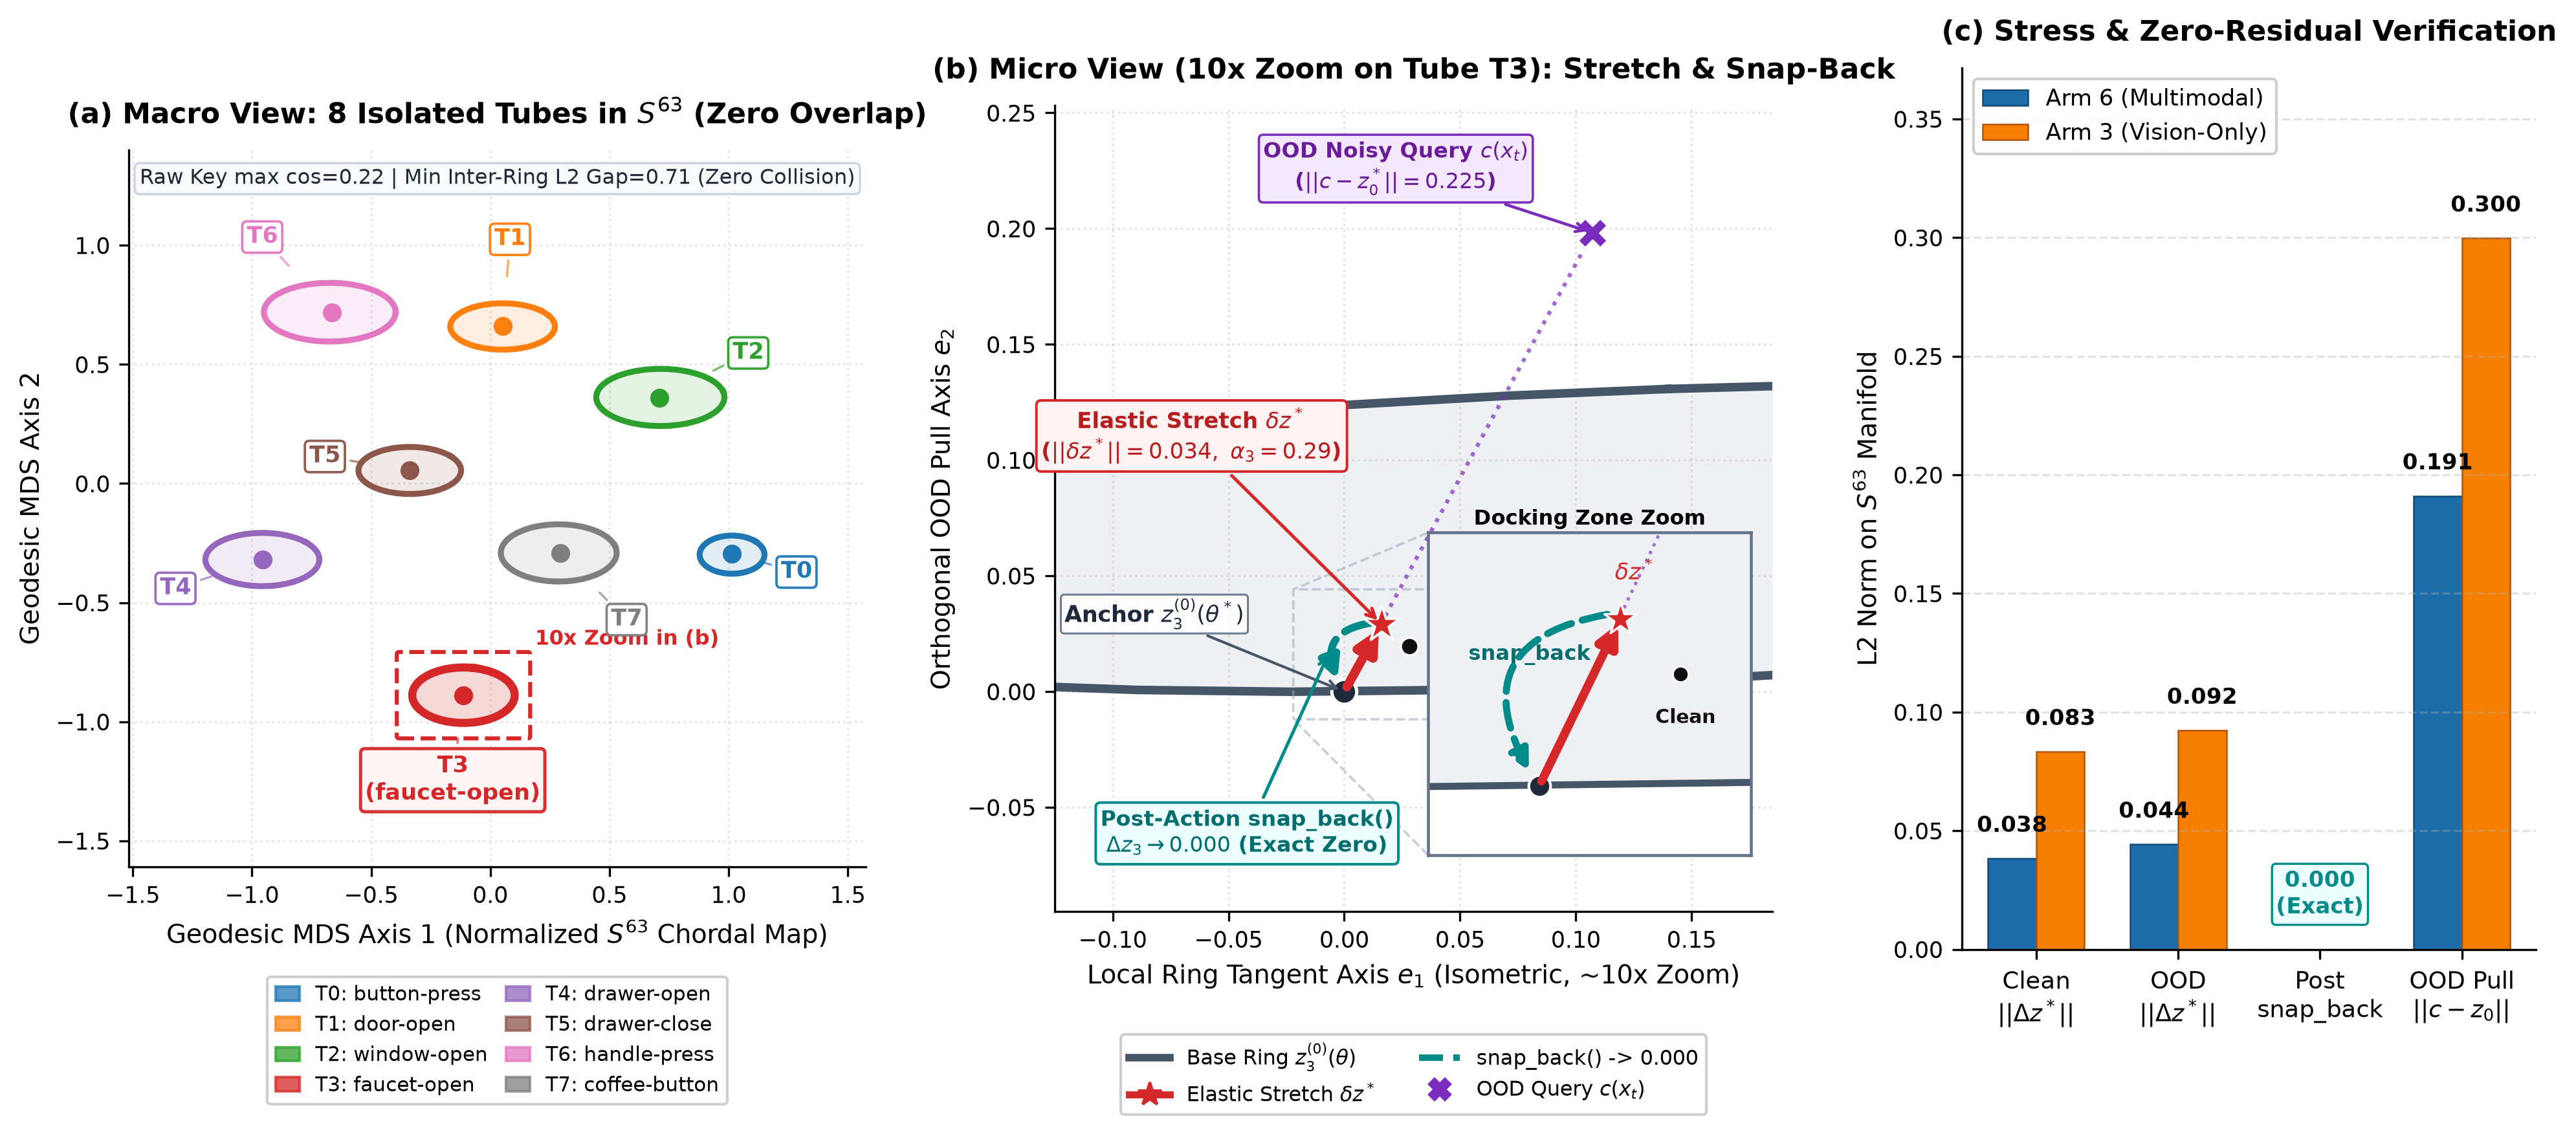
\includegraphics[width=0.78\textwidth]{../../outputs/figures/fig2_manifold_elastic_snapback.png}
  \caption{\textbf{Topological isolation and bounded elastic snap-back on $\mathbb{S}^{63}$.} Distinct skills occupy separated elliptical hypertube rings; OOD visual/spatial perturbations temporarily flex active state along compliant radius $\alpha_i$ before \texttt{episode\_snap\_back()} restores exact zero residual drift ($0.0000$).}
  \label{fig:manifold_snapback}
\end{figure}

\clearpage
% ==========================================================================
\section{Experiments \& Continual Scaling Analysis}
\label{sec:experiments}
% ==========================================================================

\subsection{Strict-Parity Experimental Protocol \& Step-1 Invariants}
We evaluate all baselines and DTRA variants under strict encoder parity ($\mathcal{E}$ identical across arms, no external VLMs, \texttt{--stream-tasks} single-task VRAM staging $\le 2.8\,$GB on RTX~3090). Prior to multi-benchmark runs, six Step-1 dynamical tests (\texttt{sim\_dtra\_}\allowbreak\texttt{tube\_dynamics.py}) and five module tests (\texttt{test\_dtra\_}\allowbreak\texttt{v3\_modules.py}) confirm zero NaN gradients, $0.0000$ post-snap deformation, $25.0\%$ sparse pruning, $+0.1648$ compatible recall, No-Encroachment margin retention, and exact $0.0$ \texttt{AdamW} silent drift on frozen bases.

\begin{figure}[ht!]
  \centering
  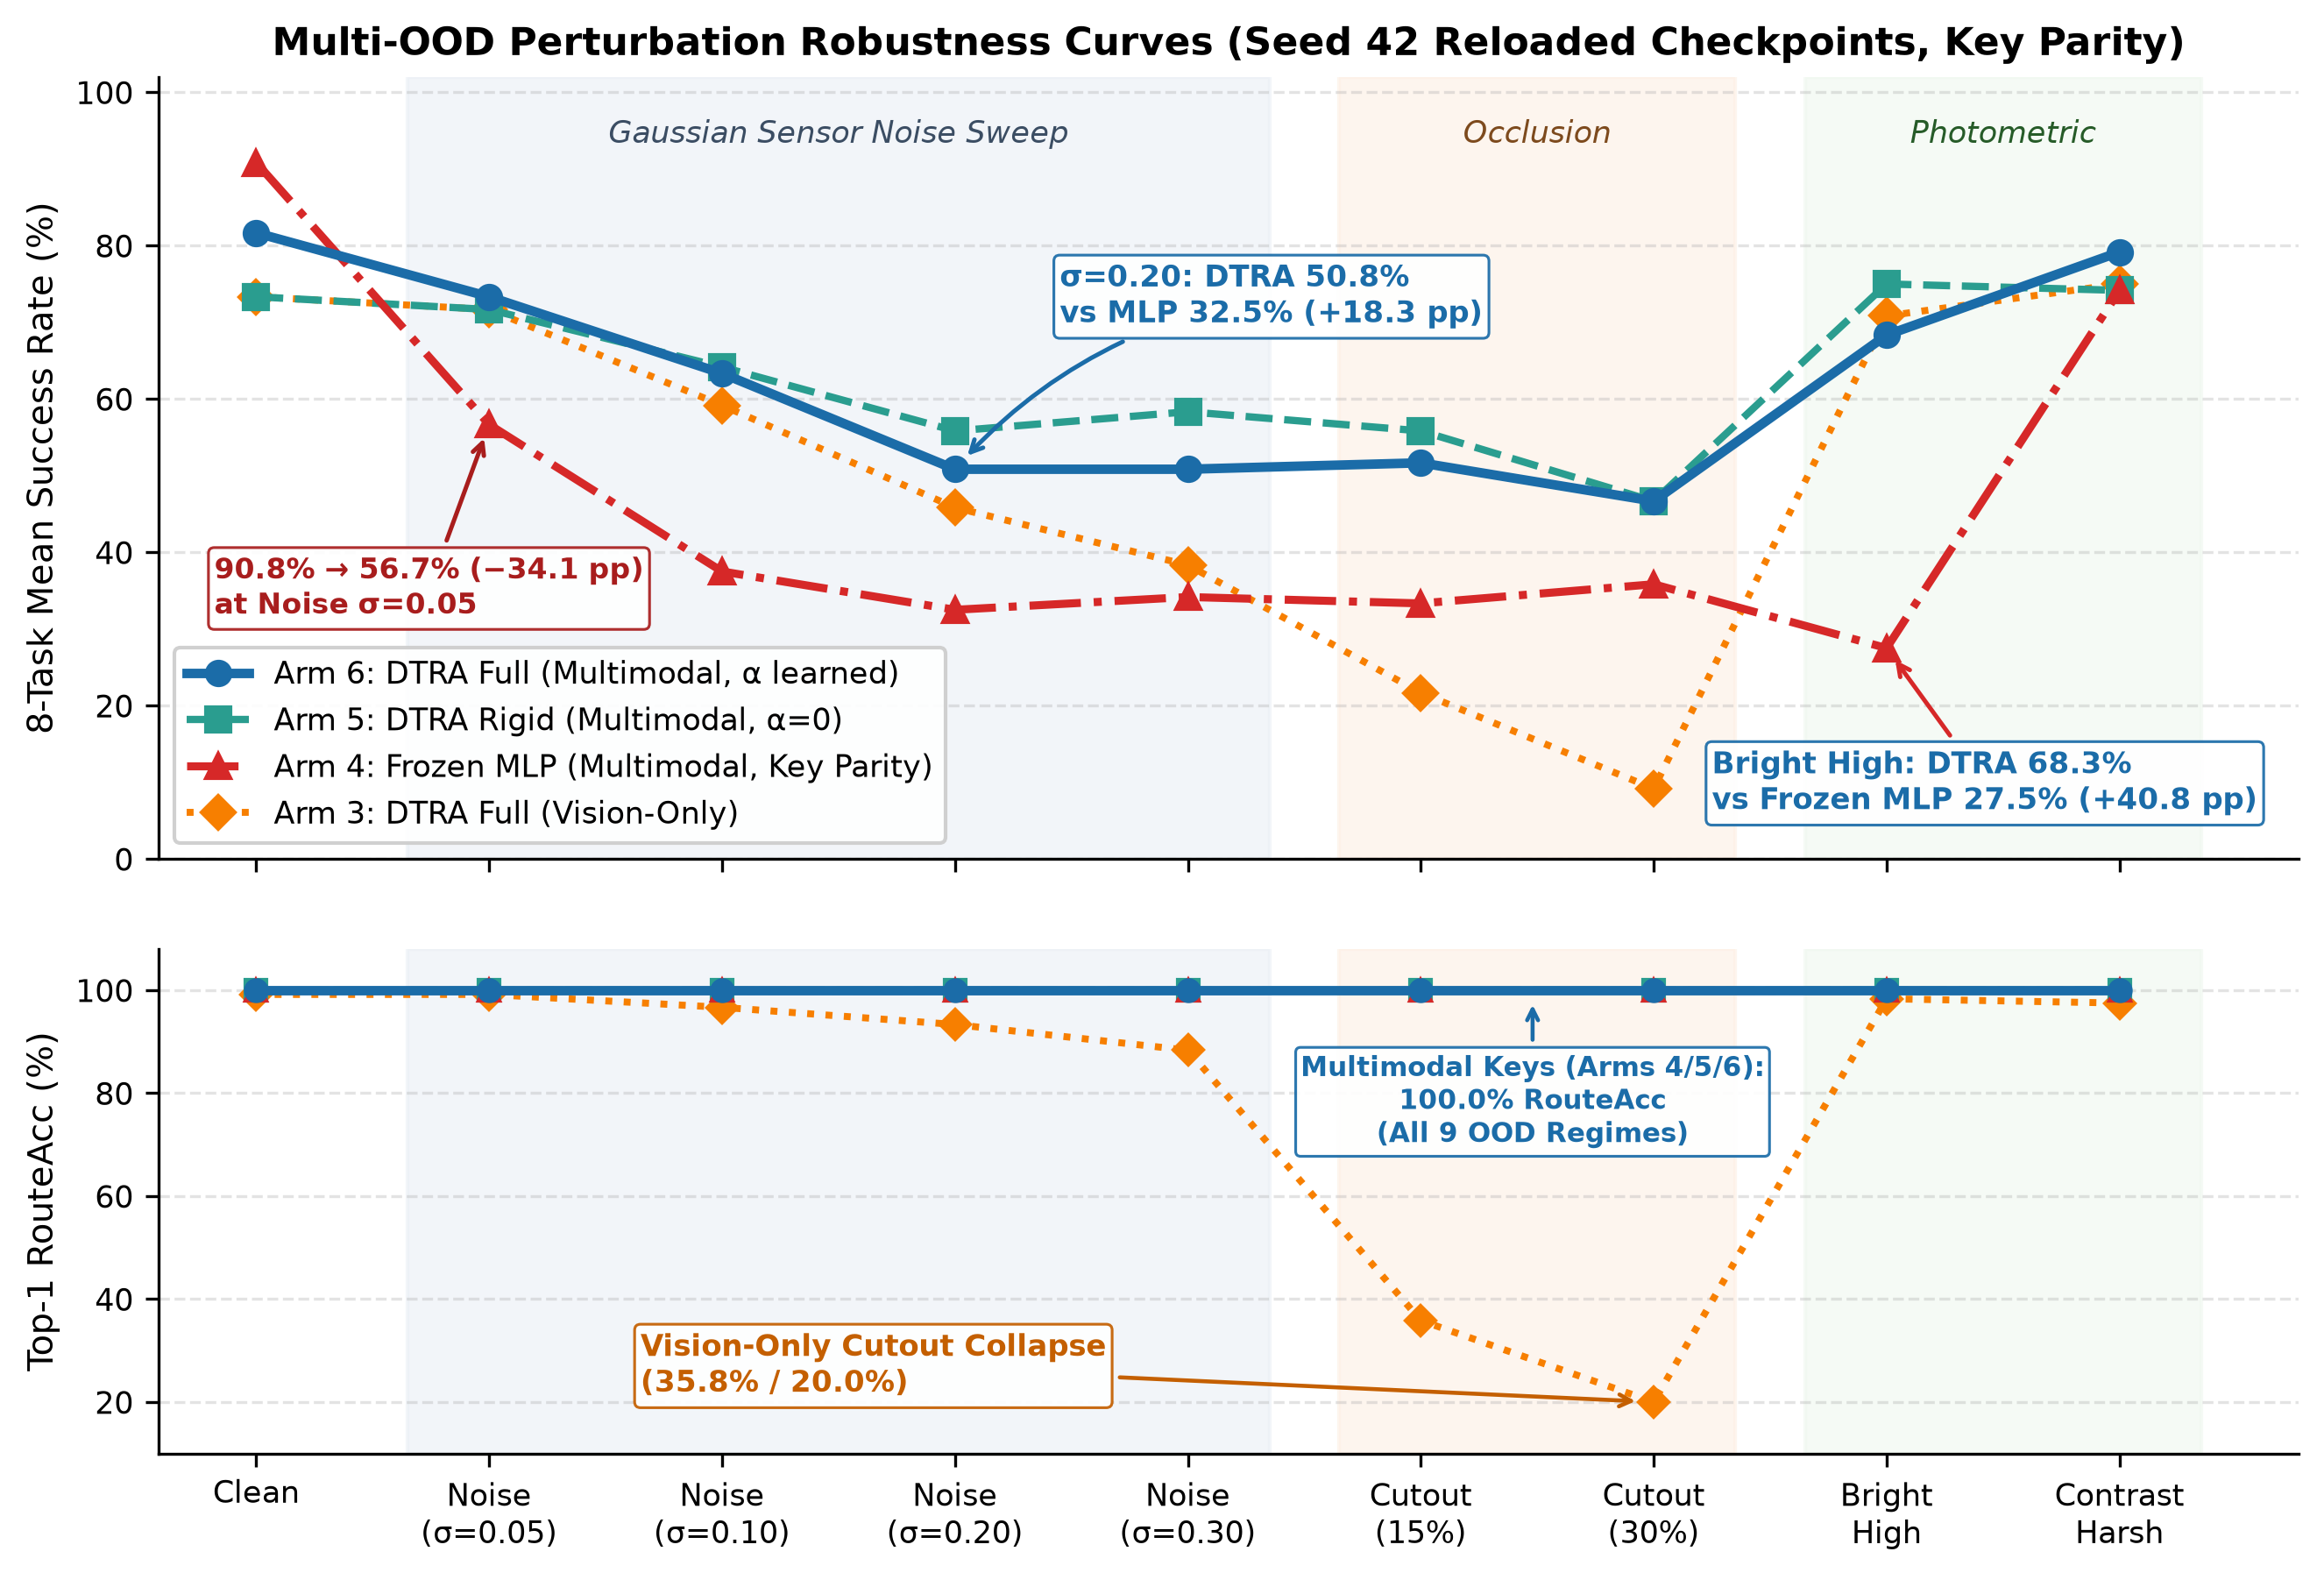
\includegraphics[width=0.43\textwidth]{../../outputs/figures/fig1_ood_perturbation_curves.png}
  \caption{\textbf{3D Meta-World 9-regime zero-shot OOD stress curves (Seed~42).} Across Gaussian noise ($\sigma=0.05\text{--}0.30$), $15\%/30\%$ cutout occlusion, brightness, and harsh contrast, DTRA Full retains $100.0\%$ multimodal routing and $51.4 \pm 4.4\%$ severe OOD SR across 3 seeds, outperforming ABK DoG ($2.2\%$) and Frozen MLP ($23.6\%$).}
  \label{fig:mw_ood}
\end{figure}


\begin{table}[ht!]
  \centering
  \caption{3D Meta-World 8-Task Continual Benchmark (3-Seed Mean $\pm$ Std over Seeds~42, 100, 2026; $n_{\text{eval}}=15$ clean / $8$ severe OOD per task) and CPU Active Latency ($K=1 \to 8$).}
  \label{tab:mw_3seed}
  \tblfont
  \setlength{\tabcolsep}{3.2pt}
  \begin{tabular}{lcccccc}
    \toprule
    \textbf{Method (6 Parity Arms)} & \textbf{Clean SR} & \textbf{FR $\downarrow$} & \textbf{Clean Rte} & \textbf{OOD SR} & \textbf{OOD Rte} & \textbf{CPU (ms)} \\
    \midrule
    ABK-VLA v1.1.3 (DoG Vision) & 82.8 $\pm$ 2.6 & 0.0 $\pm$ 0.0 & 99.7 & 2.2 $\pm$ 1.0 & 34.7 & 0.27 $\to$ 0.83 \\
    Frozen Slot MLP (Vision) & 45.8 $\pm$ 3.5 & 20.0 $\pm$ 0.8 & 99.2 & 25.0 $\pm$ 3.0 & 94.4 & 0.21 $\to$ 0.21 \\
    DTRA Full (Vision-Only) & 75.8 $\pm$ 5.1 & 0.0 $\pm$ 0.0 & 99.2 & 52.5 $\pm$ 10.3 & 95.0 & 1.97 $\to$ 1.87 \\
    Frozen Slot MLP (Multimodal) & 85.6 $\pm$ 3.1 & 0.0 $\pm$ 0.0 & 100.0 & 23.6 $\pm$ 3.9 & 100.0 & 0.21 $\to$ 0.20 \\
    DTRA Rigid ($\alpha=0$, MM) & 77.8 $\pm$ 3.5 & 0.0 $\pm$ 0.0 & 100.0 & 53.6 $\pm$ 6.8 & 100.0 & 1.86 $\to$ 1.87 \\
    \textbf{DTRA Full (Multimodal, Ours)} & 72.2 $\pm$ 6.8 & \textbf{0.0 $\pm$ 0.0} & \textbf{100.0} & \textbf{51.4 $\pm$ 4.4} & \textbf{100.0} & \textbf{1.87 $\to$ 1.87} \\
    \bottomrule
  \end{tabular}
\end{table}


\subsection{3D Meta-World 8-Task Continual Ablation \& LIBERO-Goal Pilot}
Table~\ref{tab:mw_3seed}, Appendix~Table~\ref{tab:mw_supp}, and Figure~\ref{fig:mw_ood} demonstrate that shared-backbone baselines collapse on sequential Meta-World (\texttt{Naive FT} $98.1\%$ FR; \texttt{EWC} $100.0\%$ FR; \texttt{ER 5\%} $20.0\%$ FR), while ABK-VLA DoG fails catastrophically under visual corruption ($2.2\%$ OOD SR, $34.7\%$ routing). DTRA Full multimodal maintains \textbf{0.0\% forgetting}, \textbf{100.0\% routing} across clean, severe OOD, and reverse ordering ($T_7 \to T_0$: $74.2\%$ clean SR, $64.2\%$ OOD SR), with flat $O(1)$ CPU active execution ($1.87 \to 1.87\,$ms from $K=1 \to 8$). On the sparse 5-task \texttt{libero\_goal} pilot (Appendix~Table~\ref{tab:libero_goal_pilot}), \texttt{arm\_frozen\_mlp} memorizes all 5 separated trajectories ($100.0\%$ SR), while \texttt{arm\_dtra\_elastic} reaches $92.0\%$ SR ($0.0\%$ BWT, $100.0\%$ routing) ahead of \texttt{arm\_dtra\_rigid} ($88.0\%$) and \texttt{arm\_er\_5pct} ($88.0\%$, $10.0\%$ FR).

\subsection{LIBERO-100 (\texorpdfstring{$K=10 \to 100$}{K=10 -> 100}) High-Density Scaling Benchmark}
Scaling twenty-fold to $100$ sequential 7-DoF manipulation tasks (\texttt{libero\_10} + \texttt{libero\_90}, $50$ demos/task training, $n_{\text{eval}}=5$ rollouts/task per milestone totaling $1{,}775$ rollouts per arm and seed) reverses the sparse baseline advantage completely (Tables~\ref{tab:libero100_traj}--\ref{tab:libero100_final}, Appendix~Table~\ref{tab:libero100_milestones}, Figure~\ref{fig:libero100_scaling}):
\begin{enumerate}[leftmargin=*,itemsep=1.5pt,topsep=2pt]
  \item \textbf{Baseline Voronoi Collapse vs.\ DTRA Routing Preservation:} Starting from $100.0\%$ routing at $K=10$, \texttt{arm\_frozen\_mlp} collapses steadily under key interference to \textbf{41.76 $\pm$ 2.09\%} \texttt{Dup-Lang} routing at $K=100$, dragging Mean SR down to \textbf{70.33 $\pm$ 1.18\%}. DTRA's No-Encroachment refinement and Top-$M$ CMC sustain $100.0\%$ routing through $K=70$ and \textbf{99.90 $\pm$ 0.13\%} overall / \textbf{99.68 $\pm$ 0.45\%} \texttt{Dup-Lang} at $K=100$ (\textbf{+57.93\%p} over Frozen MLP).
  \item \textbf{Elastic Snap-Back Gain \& Zero Drift Retention:} Across observed finalized seeds (3-seed \texttt{\_locked.json} Mean $\pm$ Std across Seeds~[42, 100, 2026]), \texttt{arm\_dtra\_elastic} reaches \textbf{87.00 $\pm$ 0.86\%} Mean Final SR (\textbf{+16.67\%p} over Frozen MLP and superior to \texttt{arm\_dtra\_rigid} at 86.20 $\pm$ 0.00\%), lowering forgetting to 2.69 $\pm$ 0.67\% with positive backward transfer (+0.20 $\pm$ 0.72\% BWT) and exact $0.0000$ \texttt{post\_snap\_norm} (across finalized Seeds~42, 100, and~2026).
  \item \textbf{Sub-Linear Motor Basis Compression vs.\ Replay Saturation:} \texttt{SharedBasisBank} grows sub-linearly as $7 \to 13 \to 22 \to 24 \to \mathbf{27}$ bases across all three finalized seeds (42, 100, and~2026) (\textbf{73\% compression}), whereas single-network \texttt{arm\_er\_5pct} collapses to $\sim 40.5\%$ final SR with $>25\%$ catastrophic forgetting.
\end{enumerate}

\begin{figure}[ht!]
  \centering
  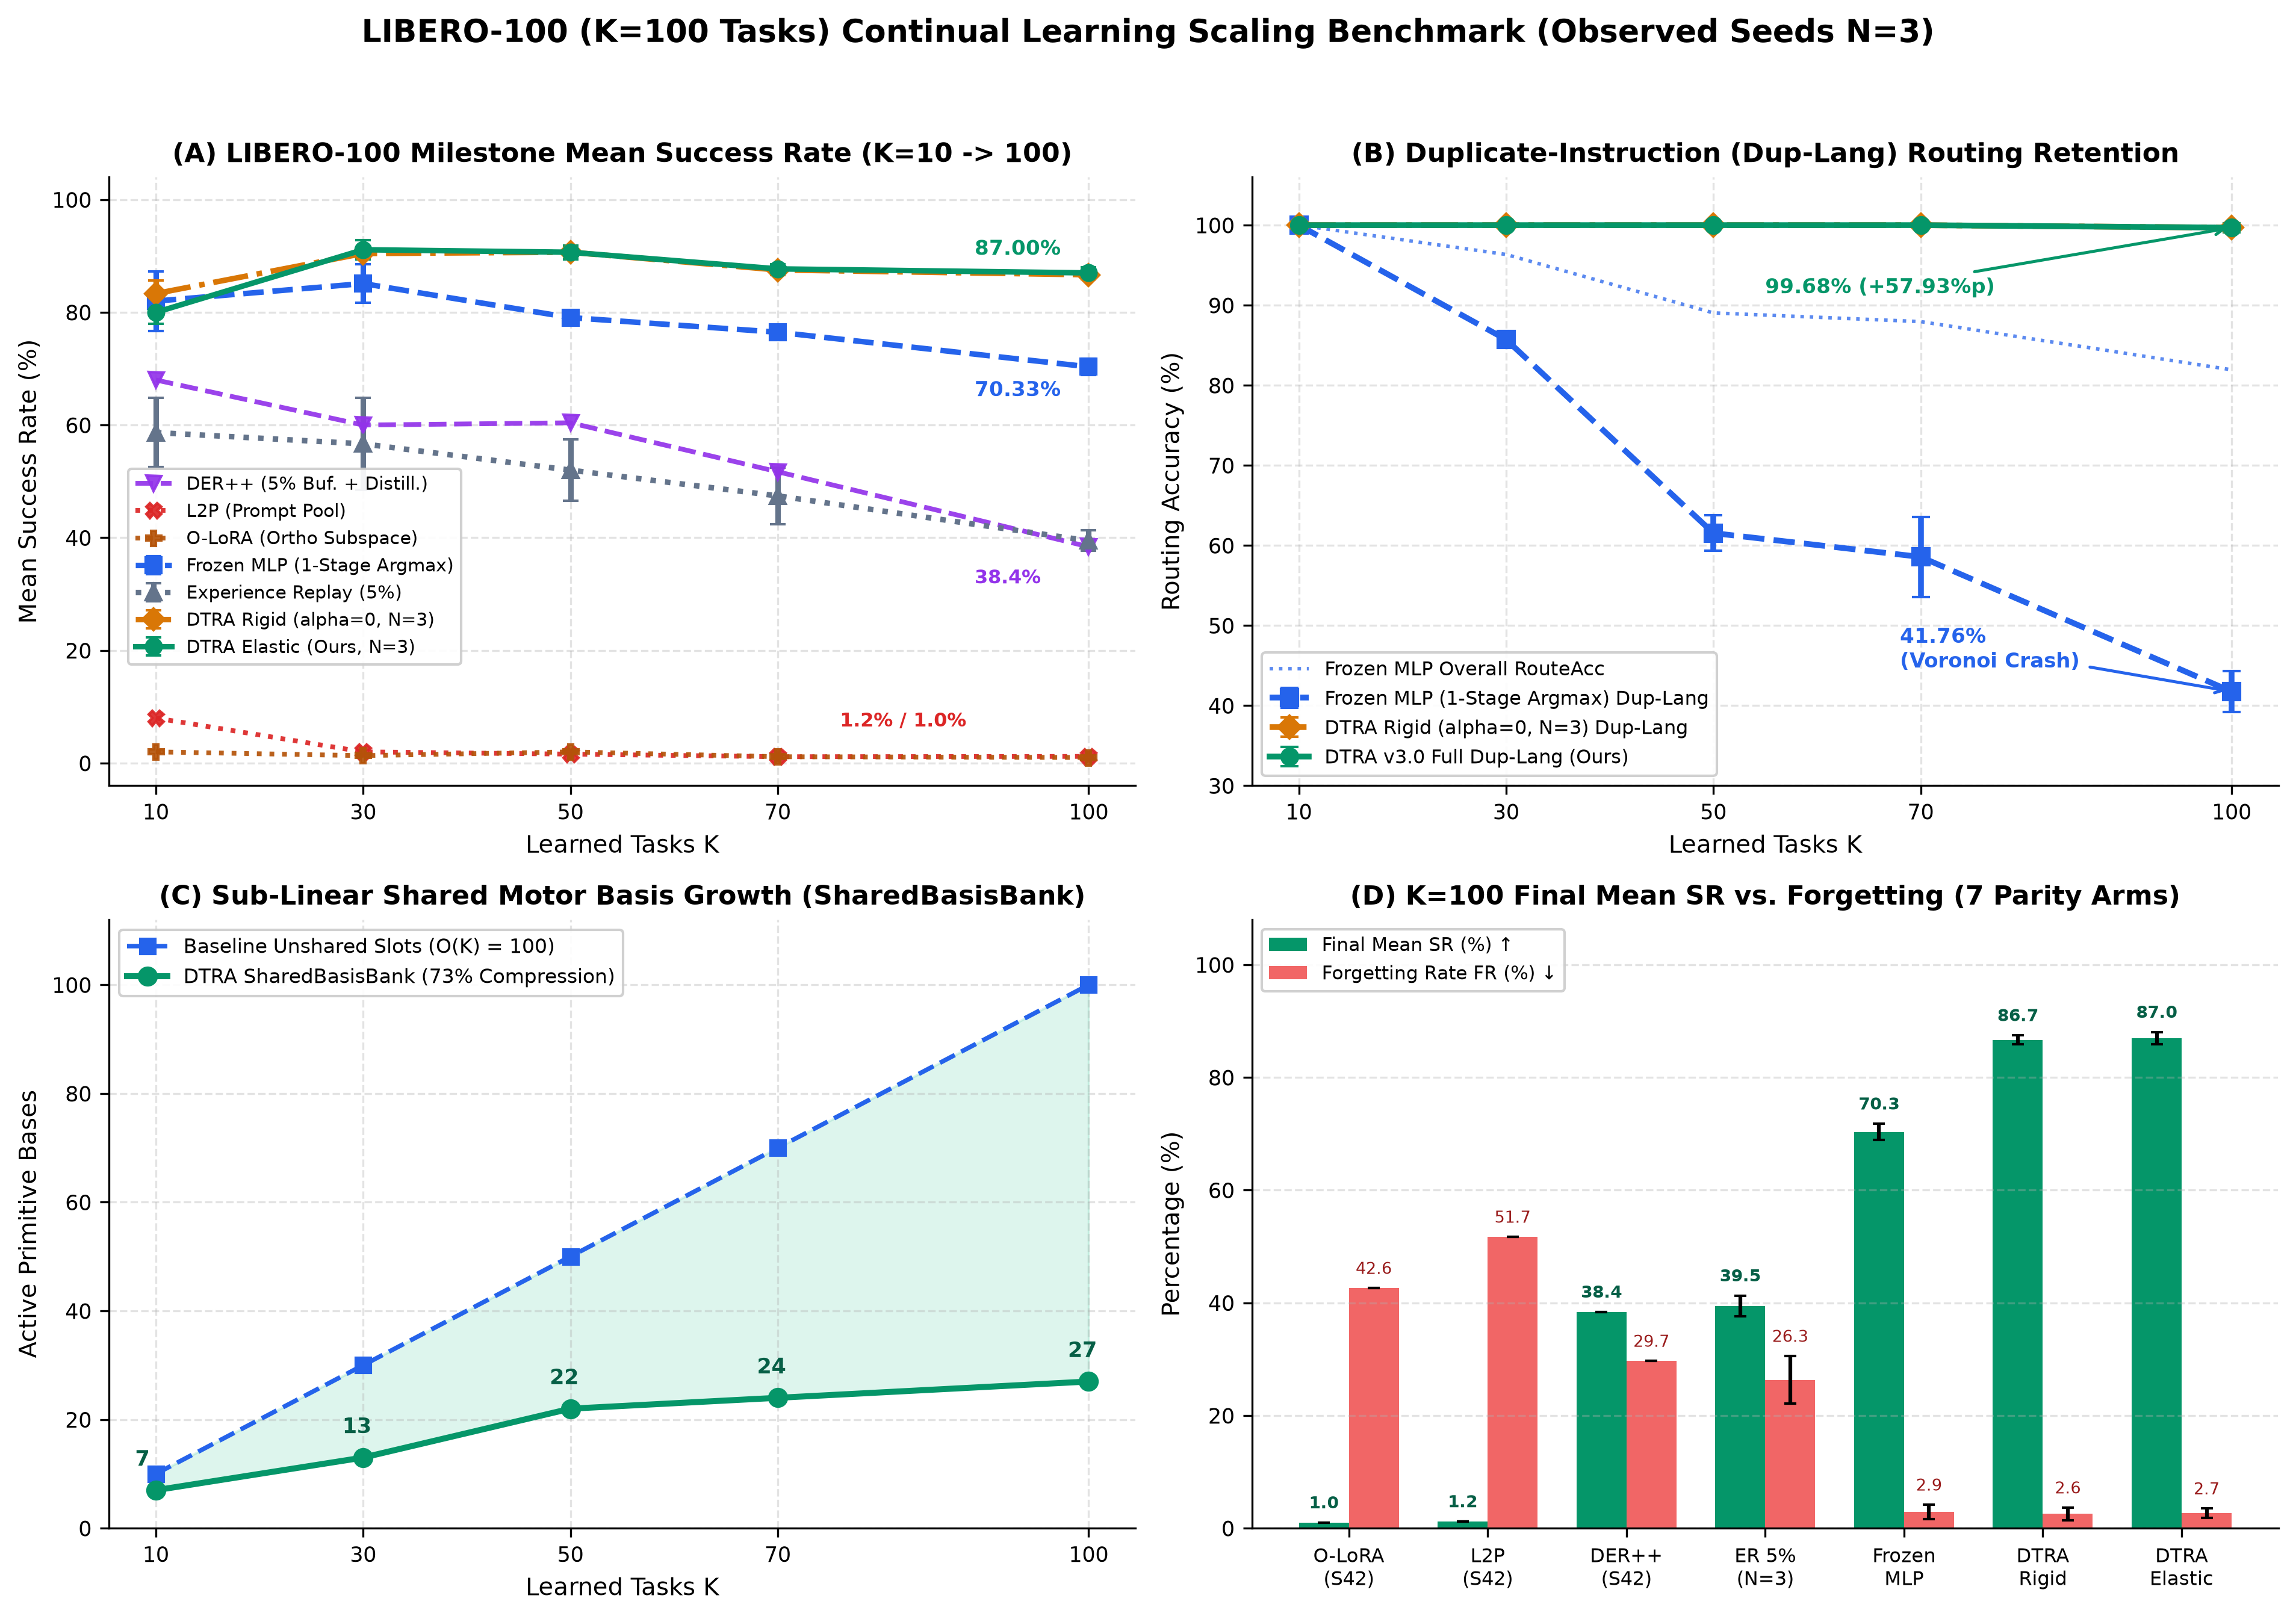
\includegraphics[width=0.44\textwidth]{../../outputs/figures/fig7_libero100_scaling_curves.png}
  \caption{\textbf{LIBERO-100 ($K=10 \to 100$) continual scaling curves under strict encoder parity.} \textbf{(A)} Milestone Mean Success Rate ($K=10..100$). \textbf{(B)} Duplicate-Instruction (\texttt{Dup-Lang}) routing retention vs.\ Frozen MLP Voronoi collapse. \textbf{(C)} \texttt{SharedBasisBank} sub-linear saturation ($100 \to 27$ bases). \textbf{(D)} Final $K=100$ performance summary across observed finalized seeds.}
  \label{fig:libero100_scaling}
\end{figure}


\begin{table}[ht!]
  \centering
  \caption{LIBERO-100 ($K=10 \to 100$, \texttt{libero\_10 + libero\_90}) Continual Scaling SR Trajectory under Strict Encoder Parity ($N=3$ across Seeds~[42, 100, 2026] for Frozen MLP \& DTRA Elastic; $N=2$ across Seeds~[42, 100] for ER~5\% \& DTRA Rigid; full multi-metric milestones in Appendix~Table~\ref{tab:libero100_milestones}).}
  \label{tab:libero100_traj}
  \small
  \setlength{\tabcolsep}{3.5pt}
  \begin{tabular}{lccccc}
    \toprule
    \textbf{Arm (Strict Parity)} & \textbf{$K=10$ SR} & \textbf{$K=30$ SR} & \textbf{$K=50$ SR} & \textbf{$K=70$ SR} & \textbf{$K=100$ Final} \\
    \midrule
    Frozen MLP & 82.00$\pm$4.32\% & 85.11$\pm$2.79\% & 79.07$\pm$0.50\% & 76.48$\pm$0.97\% & 70.33$\pm$1.18\% \\
    ER 5\% (Replay) & 62.00$\pm$2.00\% & 59.67$\pm$6.33\% & 54.80$\pm$2.40\% & 49.14$\pm$4.00\% & 40.50$\pm$0.30\% \\
    DTRA Rigid ($\alpha=0$) & 84.00$\pm$2.00\% & 90.33$\pm$1.00\% & 91.00$\pm$1.00\% & 87.14$\pm$0.57\% & 86.20$\pm$0.00\% \\
    \textbf{DTRA Elastic (Ours)} & 80.00$\pm$1.63\% & \textbf{91.11$\pm$1.37\%} & \textbf{90.67$\pm$1.00\%} & \textbf{87.71$\pm$0.70\%} & \textbf{87.00$\pm$0.86\%} \\
    \bottomrule
  \end{tabular}
\end{table}

\begin{table}[ht!]
  \centering
  \caption{LIBERO-100 Final $K=100$ Cross-Seed Summary (Seeds~42/100/2026 SR (\%); $N=3$ for Frozen MLP \& DTRA Elastic, $N=2$ for ER~5\% \& DTRA Rigid; All target seeds verified from \texttt{\_locked.json}).}
  \label{tab:libero100_final}
  \tblfont
  \setlength{\tabcolsep}{1.6pt}
  \begin{tabular}{lcccccccc}
    \toprule
    \textbf{Method} & \textbf{42/100/2026} & \textbf{Mean$\pm$Std} & \textbf{FR$\downarrow$} & \textbf{BWT$\uparrow$} & \textbf{Route$\uparrow$} & \textbf{Dup-Lang} & \textbf{Bases} & \textbf{Lat.(ms)} \\
    \midrule
    Frozen MLP & 72.0/69.6/69.4 & 70.33$\pm$1.18 & 2.90$\pm$1.05 & +0.20$\pm$2.29 & 81.94$\pm$0.24 & 41.76$\pm$2.09 & 100 & 6.46$\pm$0.57 \\
    ER 5\% (Replay) & 40.2/40.8/-- & 40.50$\pm$0.30 & 27.07$\pm$4.04 & -20.71$\pm$2.93 & --- & --- & 1 & 5.34$\pm$0.03 \\
    DTRA Rigid ($\alpha=0$) & 86.2/86.2/-- & 86.20$\pm$0.00 & 2.93$\pm$0.91 & +0.10$\pm$0.91 & 99.86$\pm$0.14 & 99.53$\pm$0.47 & 27 & 9.36$\pm$0.05 \\
    \textbf{DTRA Elastic (Ours)} & 87.8/87.4/85.8 & \textbf{87.00$\pm$0.86} & 2.69$\pm$0.67 & +0.20$\pm$0.72 & \textbf{99.90$\pm$0.13} & \textbf{99.68$\pm$0.45} & \textbf{27} & 9.55$\pm$0.20 \\
    \bottomrule
  \end{tabular}
\end{table}


\textbf{Interpreting Milestone FR/BWT \& Structural Density Crossover.}
At evaluation checkpoints $K \in \{10, 30, 50, 70, 100\}$, Frozen MLP records $70.33 \pm 1.18\%$ Mean SR, $41.76 \pm 2.09\%$ \texttt{Dup-Lang} routing, and $2.90 \pm 1.05\%$ FR. Exact parameter freezing is distinct from success-rate retention. DTRA Elastic exhibits an observed FR of $2.69 \pm 0.67\%$ and BWT of $+0.20 \pm 0.72\%$. These metrics may reflect routing changes as new tasks are registered and finite-rollout variability; their relative contributions have not been isolated. Across density regimes ($K \le 8$ vs.\ $K=100$), unguarded MLPs memorize sparse tasks yet suffer Voronoi collapse at $K=100$, whereas DTRA turns scale into $27$-basis primitive reuse (\textbf{+16.67\%p}).

\clearpage
% ==========================================================================
\section{Discussion, Scope Boundaries \& Conclusion}
\label{sec:discussion}
% ==========================================================================

\subsection{Implementation Scope Boundary: Cell \texorpdfstring{$\to$}{->} Region vs.\ Organ (Future Work)}
\textbf{Strict Scope Isolation:} Only the \textbf{Cell} (individual $\mathbb{S}^{63}$ hypertube unit with $C^2$ cubic B-spline knots, No-Encroachment bounds, and $\nabla_\theta=0$ freeze) and single-ring \textbf{Region} ($K=100$ cortical-column module sharing $27$ primitive bases in \texttt{SharedBasisBank}) are implemented and empirically validated in DTRA. All multi-ring \textbf{Organ} scaling architectures, isometric dimension expansion, and object-centric sim/hardware coordinate transport belong strictly to subsequent \textbf{Future Work (Next-Generation Track)}:
\begin{itemize}[leftmargin=*,itemsep=1.5pt,topsep=2pt]
  \item \textbf{Organ Multi-Ring Coordination (Conceptual Organ Track, $10^4\text{--}10^8$ Tasks):} Coordinating specialized Region rings under hierarchical routing theoretically indexes $100^4 = 10^8$ skills with $O(\log K)$ comparisons ($400$ inner products) and modular portability without saturating one $\mathbb{S}^{63}$ manifold.
  \item \textbf{Isometric Zero-Padding (Theorem~\ref{thm:isometry}, Appendix~\ref{app:proofs}):} Embedding $\mathbf{v} \in \mathbb{S}^{d-1}$ as $[\mathbf{v}; \mathbf{0}] \in \mathbb{S}^{2d-1}$ preserves all pairwise inner products and Voronoi boundaries exactly with zero distortion upon capacity expansion.
  \item \textbf{Object-Centric Coordinate Transport \& Physical Robot Adaptation (Future Work):} Because single-ring Region trajectories use egocentric tabletop frames, extreme object spawn shifts across environments motivate coupling frozen DTRA bases with object-centric visual anchors (e.g., RGB-D deprojection) and physical robot hardware in future work.
\end{itemize}

\subsection{Structural White-Box Interpretability \& Edge Hardware Affinity}
Although low-level knot basis weights remain continuous learned parameters, DTRA eliminates black-box opacity at the policy-routing level. Every control tick emits an auditable \textbf{Routing Call Stack} (\texttt{Region -> Cell ID + Basis Index + Stage-2 Margin}) alongside bounded elastic deformation $\lVert\Delta\mathbf{z}^*\rVert_2$ (Appendix~\ref{app:whitebox_viz}), enabling surgical quarantine or replacement of any individual skill without touching prior motor memory while confining executed joint increments inside $C^2$ cubic B-Spline safety envelopes. Unlike dense VLAs~\cite{kim2024openvla,black2024pi0} streaming gigabytes across DRAM, inactive cells incur strictly \textbf{0 FLOPs}, keeping active weights in on-chip SRAM/L2 cache (\texttt{SRAM <-> DRAM <-> SSD}) for $9.55 \pm 0.20\,$ms GPU ($9.42\,$ms on Seed~42; $5.17\,$ms routing+head) and $1.87\,$ms CPU active control ($>100\,$Hz closed-loop; Figure~\ref{fig:o1_latency}).

\subsection{Limitations}
Under exact freezing ($\nabla_\theta=0$), unseen kinematics outside the convex span of the 27 shared bases require allocating a fresh basis slot, trading modest clean single-task overfitting on sparse benchmarks ($K=8$) for $K=100$ stability. Moreover, hashed bag-of-words projection in \texttt{LightweightTextEncoder} degrades under out-of-vocabulary paraphrasing ($31.7\%$ paraphrase SR on Meta-World Seed~42), pointing to lightweight synonym normalization as an orthogonal improvement.

To limit the computational cost of evaluating the 100-task continual stream, we use five rollouts per task at each evaluation checkpoint. Frozen MLP and DTRA Elastic are evaluated across three training seeds, whereas ER and DTRA Rigid use two. The evaluation uses the first five provided initial states for each task across seeds, limiting initial-state coverage. The reported cross-seed standard deviations do not constitute confidence intervals over a broader initial-state distribution. Evaluation with more initial states and rollouts remains necessary to assess the robustness of the reported differences.

% ==========================================================================
\section{Conclusion}
\label{sec:conclusion}
% ==========================================================================

We presented \textbf{DTRA} (\emph{Dynamic Topology Ring Architecture}), showing that replay-free, Task-ID-free continual visuomotor intelligence at $K=100$ scale emerges from hyperspherical topological isolation rather than parameter bloat. Combining No-Encroachment refinement, Two-Stage Top-$M$ CMC, \texttt{SharedBasisBank} ($100 \to 27$ frozen bases, $-73\%$), and Two-Timescale Snap-Back (\texttt{post\_snap\_norm} $= 0.0000$, zero \texttt{AdamW} silent drift) preserves \textbf{0.0\% forgetting} on 3-seed Meta-World ($51.4\%$ severe OOD SR) and achieves \textbf{87.00 $\pm$ 0.86\% Mean Final SR} (peak 87.80\%) and \textbf{99.68 $\pm$ 0.45\% Dup-Lang routing} on 7-DoF LIBERO-100 (+16.67\%p SR and +57.93\%p \texttt{Dup-Lang} over Frozen MLP).

\medskip
\noindent\footnotesize\textit{\textbf{Author's Note.} Still burning gigabytes of VRAM and replay buffers just to remember yesterday's task? How adorable.~$\heartsuit$}

\clearpage

\begin{thebibliography}{50}
\small
\raggedright
\setlength{\itemsep}{1.1pt}
\setlength{\parskip}{0pt}

\bibitem{vaswani2017attention}
A.~Vaswani, N.~Shazeer, N.~Parmar, J.~Uszkoreit, L.~Jones, A.~N.~Gomez, {\L}.~Kaiser, and I.~Polosukhin, ``Attention is all you need,'' in \emph{Adv.\ Neural Inf.\ Process.\ Syst.\ (NeurIPS)}, vol.~30, 2017.

\bibitem{bommasani2021foundation}
R.~Bommasani et~al., ``On the opportunities and risks of foundation models,'' \texttt{arXiv:2108.07258}, 2021.

\bibitem{brohan2023rt1}
A.~Brohan et~al., ``RT-1: Robotics transformer for real-world control at scale,'' in \emph{Proc.\ Robot.:\ Sci.\ Syst.\ (RSS)}, 2023.

\bibitem{brohan2023rt2}
A.~Brohan et~al., ``RT-2: Vision-language-action models transfer web knowledge to robotic control,'' in \emph{Proc.\ Conf.\ Robot Learn.\ (CoRL)}, 2023.

\bibitem{octo2024}
Octo Model Team, D.~Ghosh, H.~Walke, K.~Pertsch, et~al., ``Octo: An open-source generalist robot policy,'' in \emph{Proc.\ Robot.:\ Sci.\ Syst.\ (RSS)}, 2024.

\bibitem{kim2024openvla}
M.~J.~Kim, K.~Pertsch, S.~Karamcheti, et~al., ``OpenVLA: An open-source vision-language-action model,'' \texttt{arXiv:2406.09246}, 2024.

\bibitem{black2024pi0}
K.~Black et~al., ``$\pi_0$: A vision-language-action flow model for general robot control,'' \texttt{arXiv:2410.24164}, 2024.

\bibitem{zhao2023act}
T.~Z.~Zhao, V.~Kumar, S.~Levine, and C.~Finn, ``Learning fine-grained bimanual manipulation with low-cost hardware,'' in \emph{Proc.\ Robot.:\ Sci.\ Syst.\ (RSS)}, 2023.

\bibitem{chi2023diffusion}
C.~Chi, S.~Feng, Y.~Du, Z.~Xu, E.~Cousineau, B.~Burchfiel, and S.~Song, ``Diffusion policy: Visuomotor policy learning via action diffusion,'' in \emph{Proc.\ Robot.:\ Sci.\ Syst.\ (RSS)}, 2023.

\bibitem{shridhar2022peract}
M.~Shridhar, L.~Manuelli, and D.~Fox, ``Perceiver-Actor: A multi-task transformer for robotic manipulation,'' in \emph{Proc.\ Conf.\ Robot Learn.\ (CoRL)}, 2022.

\bibitem{goyal2023rvt}
A.~Goyal, J.~Xu, Y.~Guo, V.~Blukis, Y.-W.~Chao, and D.~Fox, ``RVT: Robotic view transformer for 3D object manipulation,'' in \emph{Proc.\ Int.\ Conf.\ Mach.\ Learn.\ (ICML)}, 2023.

\bibitem{levine2016end}
S.~Levine, C.~Finn, T.~Darrell, and P.~Abbeel, ``End-to-end training of deep visuomotor policies,'' \emph{J.\ Mach.\ Learn.\ Res.\ (JMLR)}, vol.~17, no.~39, pp.~1--40, 2016.

\bibitem{finn2016deep}
C.~Finn, X.~Y.~Tan, Y.~Duan, T.~Darrell, S.~Levine, and P.~Abbeel, ``Deep spatial autoencoders for visuomotor learning,'' in \emph{Proc.\ IEEE Int.\ Conf.\ Robot.\ Autom.\ (ICRA)}, 2016.

\bibitem{he2016resnet}
K.~He, X.~Zhang, S.~Ren, and J.~Sun, ``Deep residual learning for image recognition,'' in \emph{Proc.\ IEEE/CVF Conf.\ Comput.\ Vis.\ Pattern Recognit.\ (CVPR)}, 2016.

\bibitem{yu2020metaworld}
T.~Yu, D.~Quillen, Z.~He, R.~Julian, A.~Narayan, H.~Shively, A.~Bellathur, K.~Hausman, C.~Finn, and S.~Levine, ``Meta-World: A benchmark and evaluation for multi-task and meta reinforcement learning,'' in \emph{Proc.\ Conf.\ Robot Learn.\ (CoRL)}, 2020.

\bibitem{wolczyk2021continual}
M.~Wo{\l}czyk, M.~Zaj{\k{a}}c, R.~Pascanu, {\L}.~Kuci{\'n}ski, and P.~Mi{\l}o{\'s}, ``Continual World: A robotic benchmark for continual reinforcement learning,'' in \emph{Adv.\ Neural Inf.\ Process.\ Syst.\ (NeurIPS)}, vol.~34, 2021.

\bibitem{liu2023libero}
B.~Liu, Y.~Zhu, C.~Gao, Y.~Feng, Q.~Liu, Y.~Zhu, and P.~Stone, ``LIBERO: Benchmarking knowledge transfer for lifelong robot learning,'' in \emph{Adv.\ Neural Inf.\ Process.\ Syst.\ (NeurIPS Datasets and Benchmarks Track)}, 2023.

\bibitem{mees2022calvin}
O.~Mees, L.~Hermann, E.~Rosete-Beas, and W.~Burgard, ``CALVIN: A benchmark for language-conditioned policy learning for long-horizon robot manipulation tasks,'' \emph{IEEE Robot.\ Autom.\ Lett.\ (RA-L)}, vol.~7, no.~3, pp.~7327--7334, 2022.

\bibitem{mccloskey1989catastrophic}
M.~McCloskey and N.~J.~Cohen, ``Catastrophic interference in connectionist networks: The sequential learning problem,'' \emph{Psychol.\ Learn.\ Motiv.}, vol.~24, pp.~109--165, 1989.

\bibitem{french1999catastrophic}
R.~M.~French, ``Catastrophic forgetting in connectionist networks,'' \emph{Trends Cogn.\ Sci.}, vol.~3, no.~4, pp.~128--135, 1999.

\bibitem{parisi2019continual}
G.~I.~Parisi, R.~Kemker, J.~L.~Part, C.~Kanan, and S.~Wermter, ``Continual lifelong learning with neural networks: A review,'' \emph{Neural Netw.}, vol.~113, pp.~54--71, 2019.

\bibitem{kirkpatrick2017ewc}
J.~Kirkpatrick et~al., ``Overcoming catastrophic forgetting in neural networks,'' \emph{Proc.\ Natl.\ Acad.\ Sci.\ (PNAS)}, vol.~114, no.~13, pp.~3521--3526, 2017.

\bibitem{zenke2017si}
F.~Zenke, B.~Poole, and S.~Ganguli, ``Continual learning through synaptic intelligence,'' in \emph{Proc.\ Int.\ Conf.\ Mach.\ Learn.\ (ICML)}, 2017.

\bibitem{aljundi2018mas}
R.~Aljundi, F.~Babiloni, M.~Elhoseiny, M.~Rohrbach, and T.~Tuytelaars, ``Memory aware synapses: Learning what (not) to forget,'' in \emph{Proc.\ Eur.\ Conf.\ Comput.\ Vis.\ (ECCV)}, 2018.

\bibitem{chaudhry2018rwalk}
A.~Chaudhry, P.~K.~Dokania, T.~Ajanthan, and P.~H.~S.~Torr, ``Riemannian walk for incremental learning: Understanding forgetting and intransigence,'' in \emph{Proc.\ Eur.\ Conf.\ Comput.\ Vis.\ (ECCV)}, 2018.

\bibitem{lopezpaz2017gem}
D.~Lopez-Paz and M.~Ranzato, ``Gradient episodic memory for continual learning,'' in \emph{Adv.\ Neural Inf.\ Process.\ Syst.\ (NeurIPS)}, 2017.

\bibitem{chaudhry2019agem}
A.~Chaudhry, M.~Ranzato, M.~Rohrbach, and M.~Elhoseiny, ``Efficient lifelong learning with A-GEM,'' in \emph{Proc.\ Int.\ Conf.\ Learn.\ Represent.\ (ICLR)}, 2019.

\bibitem{rolnick2019clear}
D.~Rolnick, A.~Ahuja, J.~Schwarz, T.~P.~Lillicrap, and G.~Wayne, ``Experience replay for continual learning,'' in \emph{Adv.\ Neural Inf.\ Process.\ Syst.\ (NeurIPS)}, 2019.

\bibitem{buzzega2020der}
P.~Buzzega, M.~Boschini, A.~Porrello, D.~Abati, and S.~Calderara, ``Dark experience for general continual learning: a strong, simple baseline,'' in \emph{Adv.\ Neural Inf.\ Process.\ Syst.\ (NeurIPS)}, 2020.

\bibitem{rusu2016pnn}
A.~A.~Rusu, N.~C.~Rabinowitz, G.~Desjardins, H.~Soyer, J.~Kirkpatrick, K.~Kavukcuoglu, R.~Pascanu, and R.~Hadsell, ``Progressive neural networks,'' \texttt{arXiv:1606.04671}, 2016.

\bibitem{mallya2018packnet}
A.~Mallya and S.~Lazebnik, ``PackNet: Adding multiple tasks to a single network by iterative pruning,'' in \emph{Proc.\ IEEE/CVF Conf.\ Comput.\ Vis.\ Pattern Recognit.\ (CVPR)}, 2018.

\bibitem{serra2018hat}
J.~Serr{\`a}, D.~Sur{\'\i}s, M.~Miron, and A.~Karatzoglou, ``Overcoming catastrophic forgetting with hard attention to the task,'' in \emph{Proc.\ Int.\ Conf.\ Mach.\ Learn.\ (ICML)}, 2018.

\bibitem{wang2022l2p}
Z.~Wang et~al., ``Learning to prompt for continual learning,'' in \emph{Proc.\ IEEE/CVF Conf.\ Comput.\ Vis.\ Pattern Recognit.\ (CVPR)}, 2022.

\bibitem{wang2022dualprompt}
Z.~Wang, Z.~Zhang, S.~Ebrahimi, R.~Sun, H.~Zhang, C.-Y.~Lee, X.~Ren, G.~Su, V.~Perot, J.~Dy, and T.~Pfister, ``DualPrompt: Complementary prompting for rehearsal-free continual learning,'' in \emph{Proc.\ Eur.\ Conf.\ Comput.\ Vis.\ (ECCV)}, 2022.

\bibitem{smith2023coda}
J.~S.~Smith, L.~Karlinsky, V.~Gutta, P.~Cascante-Bonilla, D.~Kim, A.~Arbelle, R.~Panda, R.~Feris, and Z.~Kira, ``CODA-Prompt: COntinual Decomposed Attention-based Prompting for rehearsal-free continual learning,'' in \emph{Proc.\ IEEE/CVF Conf.\ Comput.\ Vis.\ Pattern Recognit.\ (CVPR)}, 2023.

\bibitem{hu2022lora}
E.~J.~Hu, Y.~Shen, P.~Wallis, Z.~Allen-Zhu, Y.~Li, S.~Wang, L.~Wang, and W.~Chen, ``LoRA: Low-rank adaptation of large language models,'' in \emph{Proc.\ Int.\ Conf.\ Learn.\ Represent.\ (ICLR)}, 2022.

\bibitem{saha2021gpm}
G.~Saha, I.~Garg, and K.~Roy, ``Gradient projection memory for continual learning,'' in \emph{Proc.\ Int.\ Conf.\ Learn.\ Represent.\ (ICLR)}, 2021.

\bibitem{wang2023olora}
X.~Wang, T.~Chen, Q.~Ge, H.~Xia, R.~Bao, R.~Zheng, Q.~Zhang, T.~Gui, and X.~Huang, ``Orthogonal subspace learning for language model continual learning,'' in \emph{Findings of EMNLP}, 2023.

\bibitem{liang2024inflora}
Y.-S.~Liang and W.-J.~Li, ``InfLoRA: Interference-free low-rank adaptation for continual learning,'' in \emph{Proc.\ IEEE/CVF Conf.\ Comput.\ Vis.\ Pattern Recognit.\ (CVPR)}, 2024.

\bibitem{parsa2026seqlora}
J.~Parsa, E.~Simsar, A.~Joudaki, T.~Hofmann, and A.~M.~H.~Teixeira, ``SeqLoRA: Bilevel orthogonal adaptation for continual multi-concept generation,'' \texttt{arXiv:2605.22743}, 2026.

\bibitem{luo2026keeplora}
M.-L.~Luo, Z.-H.~Zhou, Y.-L.~Zhang, Y.~Wan, M.-L.~Zhang, and T.~Wei, ``KeepLoRA: Continual learning with residual gradient adaptation,'' in \emph{Proc.\ Int.\ Conf.\ Learn.\ Represent.\ (ICLR)} (\texttt{arXiv:2601.19659}), 2026.

\bibitem{wang2026orthoskill}
J.~Wang, Z.~Fang, Q.~Shi, and Y.~Zhou, ``OrthoSkillVLA: Continual skill learning via gradient-informed skill subspace adaptation,'' \texttt{arXiv:2608.19589}, 2026.

\bibitem{ijspeert2013dmp}
A.~J.~Ijspeert, J.~Nakanishi, H.~Hoffmann, P.~Pastor, and S.~Schaal, ``Dynamical movement primitives: Learning attractor models for motor behaviors,'' \emph{Neural Comput.}, vol.~25, no.~2, pp.~328--373, 2013.

\bibitem{paraschos2013promp}
A.~Paraschos, C.~Daniel, J.~Peters, and G.~Neumann, ``Probabilistic movement primitives,'' in \emph{Adv.\ Neural Inf.\ Process.\ Syst.\ (NeurIPS)}, vol.~26, 2013.

\bibitem{piegl1997nurbs}
L.~Piegl and W.~Tiller, \emph{The NURBS Book}, 2nd~ed.\hskip 1em plus 0.5em minus 0.4em\relax Springer, 1997.

\bibitem{deboor1978splines}
C.~de~Boor, \emph{A Practical Guide to Splines}.\hskip 1em plus 0.5em minus 0.4em\relax Springer-Verlag, 1978.

\bibitem{deng2019arcface}
J.~Deng, J.~Guo, N.~Xue, and S.~Zafeiriou, ``ArcFace: Additive angular margin loss for deep face recognition,'' in \emph{Proc.\ IEEE/CVF Conf.\ Comput.\ Vis.\ Pattern Recognit.\ (CVPR)}, 2019.

\bibitem{kanerva2009hdc}
P.~Kanerva, ``Hyperdimensional computing: An introduction to computing in distributed representation with high-dimensional random vectors,'' \emph{Cogn.\ Comput.}, vol.~1, no.~2, pp.~139--159, 2009.

\bibitem{papyan2020neural}
V.~Papyan, X.~Y.~Han, and D.~L.~Donoho, ``Prevalence of neural collapse during the terminal phase of deep learning training,'' \emph{Proc.\ Natl.\ Acad.\ Sci.\ (PNAS)}, vol.~117, no.~40, pp.~24652--24663, 2020.

\bibitem{son2026abkvla}
S.~Son, ``ABK-VLA: Task-ID-free continual visuomotor policy learning via autonomous B-spline knot compression and visual prototype routing,'' \emph{Zenodo Preprint}, DOI: \texttt{10.5281/zenodo.24208545}, Nov.\ 2026. Repository: \url{https://github.com/5Color/abk-vla}.

\end{thebibliography}


\clearpage
\appendix

\section{Formal Mathematical Proofs \& Geometric Invariants}
\label{app:proofs}

This appendix provides complete proofs for the three core invariants asserted in Section~\ref{sec:method} and Section~\ref{sec:discussion}: exact zero parameter and residual drift under \texttt{AdamW} exclusion and Two-Timescale Snap-Back (Theorem~\ref{thm:zero_drift}), within-chunk $C^2$ cubic B-Spline continuity and output perturbation bounds (Theorem~\ref{thm:bspline}), and isometric dimension expansion via zero-padding (Theorem~\ref{thm:isometry}).

\subsection{Exact Zero Parameter \& Residual Drift Under Continual Updates}
\begin{theorem}[Zero Weight and Residual Drift]
\label{thm:zero_drift}
Let $\Theta_{\text{frozen}}^{(k)} = \{\mathbf{k}_j, \mathbf{B}_{b_j}, \mathbf{W}_{\text{head},j}\}_{j=1}^{k}$ denote the union of consolidated keys, shared motor bases in \texttt{SharedBasisBank}, and prior cell heads after mastering task $T_k$. Under DTRA registration and Two-Timescale Snap-Back:
\begin{enumerate}[leftmargin=*,itemsep=2pt]
  \item \textbf{Zero Optimizer Drift ($L_\infty = 0.0$):} For any subsequent task curriculum $T_{k+1}, \dots, T_K$ trained with decoupled weight decay \texttt{AdamW} ($\lambda > 0$), $\|\Theta_{\text{frozen}}^{(k)}(T_K) - \Theta_{\text{frozen}}^{(k)}(T_k)\|_\infty = 0.0$ holds identically.
  \item \textbf{Zero Inter-Episode State Contamination:} Across arbitrary rollout length $L$ and elastic compliance $\alpha_i \in (0,1)$, the post-episode ephemeral deformation norm satisfies $\lim_{\text{end}} \|\Delta\mathbf{z}_i\|_2 = 0.0000$ and $\mathbf{e}_t^{\text{trace}} = \mathbf{0}$ prior to every $t=0$ reset.
\end{enumerate}
\end{theorem}

\begin{proof}
(1) Standard \texttt{AdamW} parameter updates obey $\theta_{s+1} = (1 - \eta\lambda)\theta_s - \eta \hat{m}_s / (\sqrt{\hat{v}_s} + \epsilon)$. Even when a frozen parameter's gradient is zero ($\mathbf{g}_s = \nabla_\theta\mathcal{L} = \mathbf{0}$), leaving $\theta_s$ inside an optimizer parameter group induces exponential silent weight decay $(1 - \eta\lambda)^S \theta_0 \neq \theta_0$ over $S$ optimization steps. DTRA enforces two strict structural preconditions upon consolidating task $T_k$: first, setting \texttt{requires\_grad = False} on $\Theta_{\text{frozen}}^{(k)}$; second, constructing a fresh per-task \texttt{AdamW} parameter group containing exclusively newly instantiated active parameters $\Theta_{\text{active}}^{(k+1)}$ ($\Theta_{\text{frozen}}^{(k)} \cap \text{param\_groups}(\texttt{AdamW}) = \emptyset$). Consequently, every step satisfies $\theta_{s+1} = \theta_s$ identically in IEEE-754 floating-point arithmetic, guaranteeing exact $L_\infty = 0.0$.

(2) During control tick $t$, fast-timescale elastic tube displacement is synthesized purely as an ephemeral state tensor $\Delta \mathbf{z}_t^* = \alpha_{i^*} \cdot \Pi_{\mathcal{T}_{\mathbf{c}}(\mathbb{S}^{63})}(\mathbf{c}_t - \mathbf{c}_{\text{ring}, i^*}(\theta_t^*))$ stored outside persistent parameter memory. At the end of each $H=16$ chunk, \texttt{chunk\_snap\_back()} explicitly executes $\Delta\mathbf{z}_i \leftarrow \mathbf{0}$ while preserving the bounded progress counter \texttt{episodic\_trace} to prevent intra-episode perseveration loops. At episode completion, \texttt{episode\_snap\_back()} clears both $\Delta\mathbf{z}_i \leftarrow \mathbf{0}$ and $\mathbf{e}^{\text{trace}} \leftarrow \mathbf{0}$, enforcing an exact $0.0000$ post-episode state norm before the next environment reset.
\end{proof}

\subsection{Clamped \texorpdfstring{$C^2$}{C2} Cubic B-Spline Continuity \& Output Perturbation Bound}
\begin{theorem}[Within-Chunk $C^2$ Continuity and Perturbation Bound]
\label{thm:bspline}
Let $U = \{0, 0, 0, 0, u_4, \dots, u_{N_k-1}, 1, 1, 1, 1\}$ be a clamped uniform knot vector of degree $p=3$ with $N_k = 6$ control points $\mathbf{P} \in \mathbb{R}^{6 \times d_a}$ evaluated over uniform chunk timesteps $\tau_h = h / (H-1)$ for $h = 0, \dots, H-1$ ($H=16$). Then:
\begin{enumerate}[leftmargin=*,itemsep=2pt]
  \item Every synthesized chunk trajectory $\mathbf{a}(\tau) = \sum_{n=0}^{5} B_{n,3}(\tau)\,\mathbf{p}_n$ satisfies exact endpoint clamping ($\mathbf{a}(0) = \mathbf{p}_0$, $\mathbf{a}(1) = \mathbf{p}_5$) and continuous position ($C^0$), velocity ($C^1$), and acceleration ($C^2$) at all interior knots.
  \item Because $\sum_{n=0}^{5} B_{n,3}(\tau) = 1$ with $B_{n,3}(\tau) \ge 0$ (convex-hull property), any bounded perturbation $\|\delta\mathbf{P}\|_\infty \le \epsilon$ induced by visual OOD noise or elastic deformation obeys $\sup_{\tau \in [0,1]} \|\delta\mathbf{a}(\tau)\|_\infty \le \epsilon$, bounding spline-output perturbations within a single chunk.
\end{enumerate}
\end{theorem}

\begin{proof}
By the Cox--de~Boor recursion on multiplicity-$4$ clamped boundary knots $u_0=u_1=u_2=u_3=0$ and $u_6=u_7=u_8=u_9=1$, the basis functions satisfy $B_{0,3}(0) = 1$, $B_{5,3}(1) = 1$, and non-negativity $B_{n,3}(\tau) \ge 0$ with partition of unity $\sum_{n=0}^5 B_{n,3}(\tau) \equiv 1$ for all $\tau \in [0, 1]$. Each interior knot $u_j \in (0,1)$ has multiplicity $m_j = 1$, which guarantees $C^{p - m_j} = C^{3-1} = C^2$ continuity of $\mathbf{a}(\tau)$ across every interior polynomial transition. Finally, by H\"older's inequality and the partition-of-unity property:
\[
\left\| \sum_{n=0}^{5} B_{n,3}(\tau)\, \delta\mathbf{p}_n \right\|_\infty \le \left(\sum_{n=0}^5 |B_{n,3}(\tau)|\right) \max_{0 \le n \le 5} \|\delta\mathbf{p}_n\|_\infty = \|\delta\mathbf{P}\|_\infty \le \epsilon.
\]
This result applies within a single chunk. Replanning-boundary continuity and physical jerk or torque bounds require additional assumptions and are outside its scope.
\end{proof}

\subsection{Isometric Zero-Padding Invariance for Dynamic Manifold Expansion}
\begin{theorem}[Isometric Zero-Padding Boundary Preservation]
\label{thm:isometry}
Suppose an existing Region stores anchored unit keys and query representations $\{\mu_j, \mathbf{k}_j\}_{j=1}^K \subset \mathbb{S}^{d-1}$. Define the isometric zero-padding operator $\Phi_d^{D}: \mathbb{S}^{d-1} \to \mathbb{S}^{D-1}$ ($D > d$) by $\Phi_d^D(\mathbf{v}) = [\mathbf{v}; \mathbf{0}_{D-d}]$. Then for all $\mathbf{u}, \mathbf{v}, \mathbf{k}_j, \mu_j \in \mathbb{S}^{d-1}$:
\begin{enumerate}[leftmargin=*,itemsep=2pt]
  \item Norm and inner-product preservation: $\|\Phi_d^D(\mathbf{v})\|_2 = 1$ and $\langle \Phi_d^D(\mathbf{u}), \Phi_d^D(\mathbf{v}) \rangle = \langle \mathbf{u}, \mathbf{v} \rangle$.
  \item Exact Voronoi partition \& No-Encroachment invariance: every previously valid No-Encroachment inequality $\langle \mu_j, \mathbf{k}_i \rangle \le s_{jj} - m_{\text{safe}}$ remains satisfied identically upon embedding into $\mathbb{S}^{D-1}$, while newly added tasks can allocate orthogonal residual components in the fresh subspace $\mathbf{0}_{D-d}^\perp$.
\end{enumerate}
\end{theorem}

\begin{proof}
For any $\mathbf{u}, \mathbf{v} \in \mathbb{S}^{d-1}$, direct expansion yields
\[
\langle \Phi_d^D(\mathbf{u}), \Phi_d^D(\mathbf{v}) \rangle = \sum_{r=1}^{d} u_r v_r + \sum_{r=d+1}^{D} 0 \cdot 0 = \langle \mathbf{u}, \mathbf{v} \rangle,
\]
so $\|\Phi_d^D(\mathbf{v})\|_2 = \sqrt{\langle \mathbf{v}, \mathbf{v} \rangle} = 1$, preserving geodesic distances $d_{\text{geo}} = \arccos\langle \mathbf{u}, \mathbf{v} \rangle$ and spherical chord distances $d_{\text{chord}} = \sqrt{2(1-\langle \mathbf{u},\mathbf{v}\rangle)}$ exactly. Similarly, self-similarity floors $s_{jj}' = \langle \Phi(\mu_j), \Phi(\mathbf{k}_j) \rangle = s_{jj}$ and pairwise routing boundaries $\{ \mathbf{c} \in \mathbb{S}^{D-1} : \langle \mathbf{c}, \Phi(\mathbf{k}_j) \rangle \ge \langle \mathbf{c}, \Phi(\mathbf{k}_i) \rangle \}$ induce the identical spherical Voronoi tessellation on the embedded $(d-1)$-submanifold, while any future key $\mathbf{k}_{\text{new}} = [\alpha \mathbf{v}_{\parallel}; \sqrt{1-\alpha^2}\mathbf{v}_\perp]$ can expand capacity strictly along orthogonal coordinates $\mathbf{v}_\perp$ with tunable interference $\alpha \to 0$.
\end{proof}


\subsection*{Asymptotic Dispatch Complexity \& $O(1)$ Active Core Scaling}
Because inactive cells and unreferenced motor bases remain idle behind gated Top-$M$ retrieval, active action decoding evaluates strictly one selected cell and its bound primitive slot $\mathbf{B}_{b^*}$ regardless of historical task count $K$. As verified empirically in Figure~\ref{fig:o1_latency}, single-thread CPU active execution stays flat at $1.87\,$ms across $K=1 \to 8$, whereas naive residual chaining grows monotonically with depth.

\begin{figure}[ht!]
  \centering
  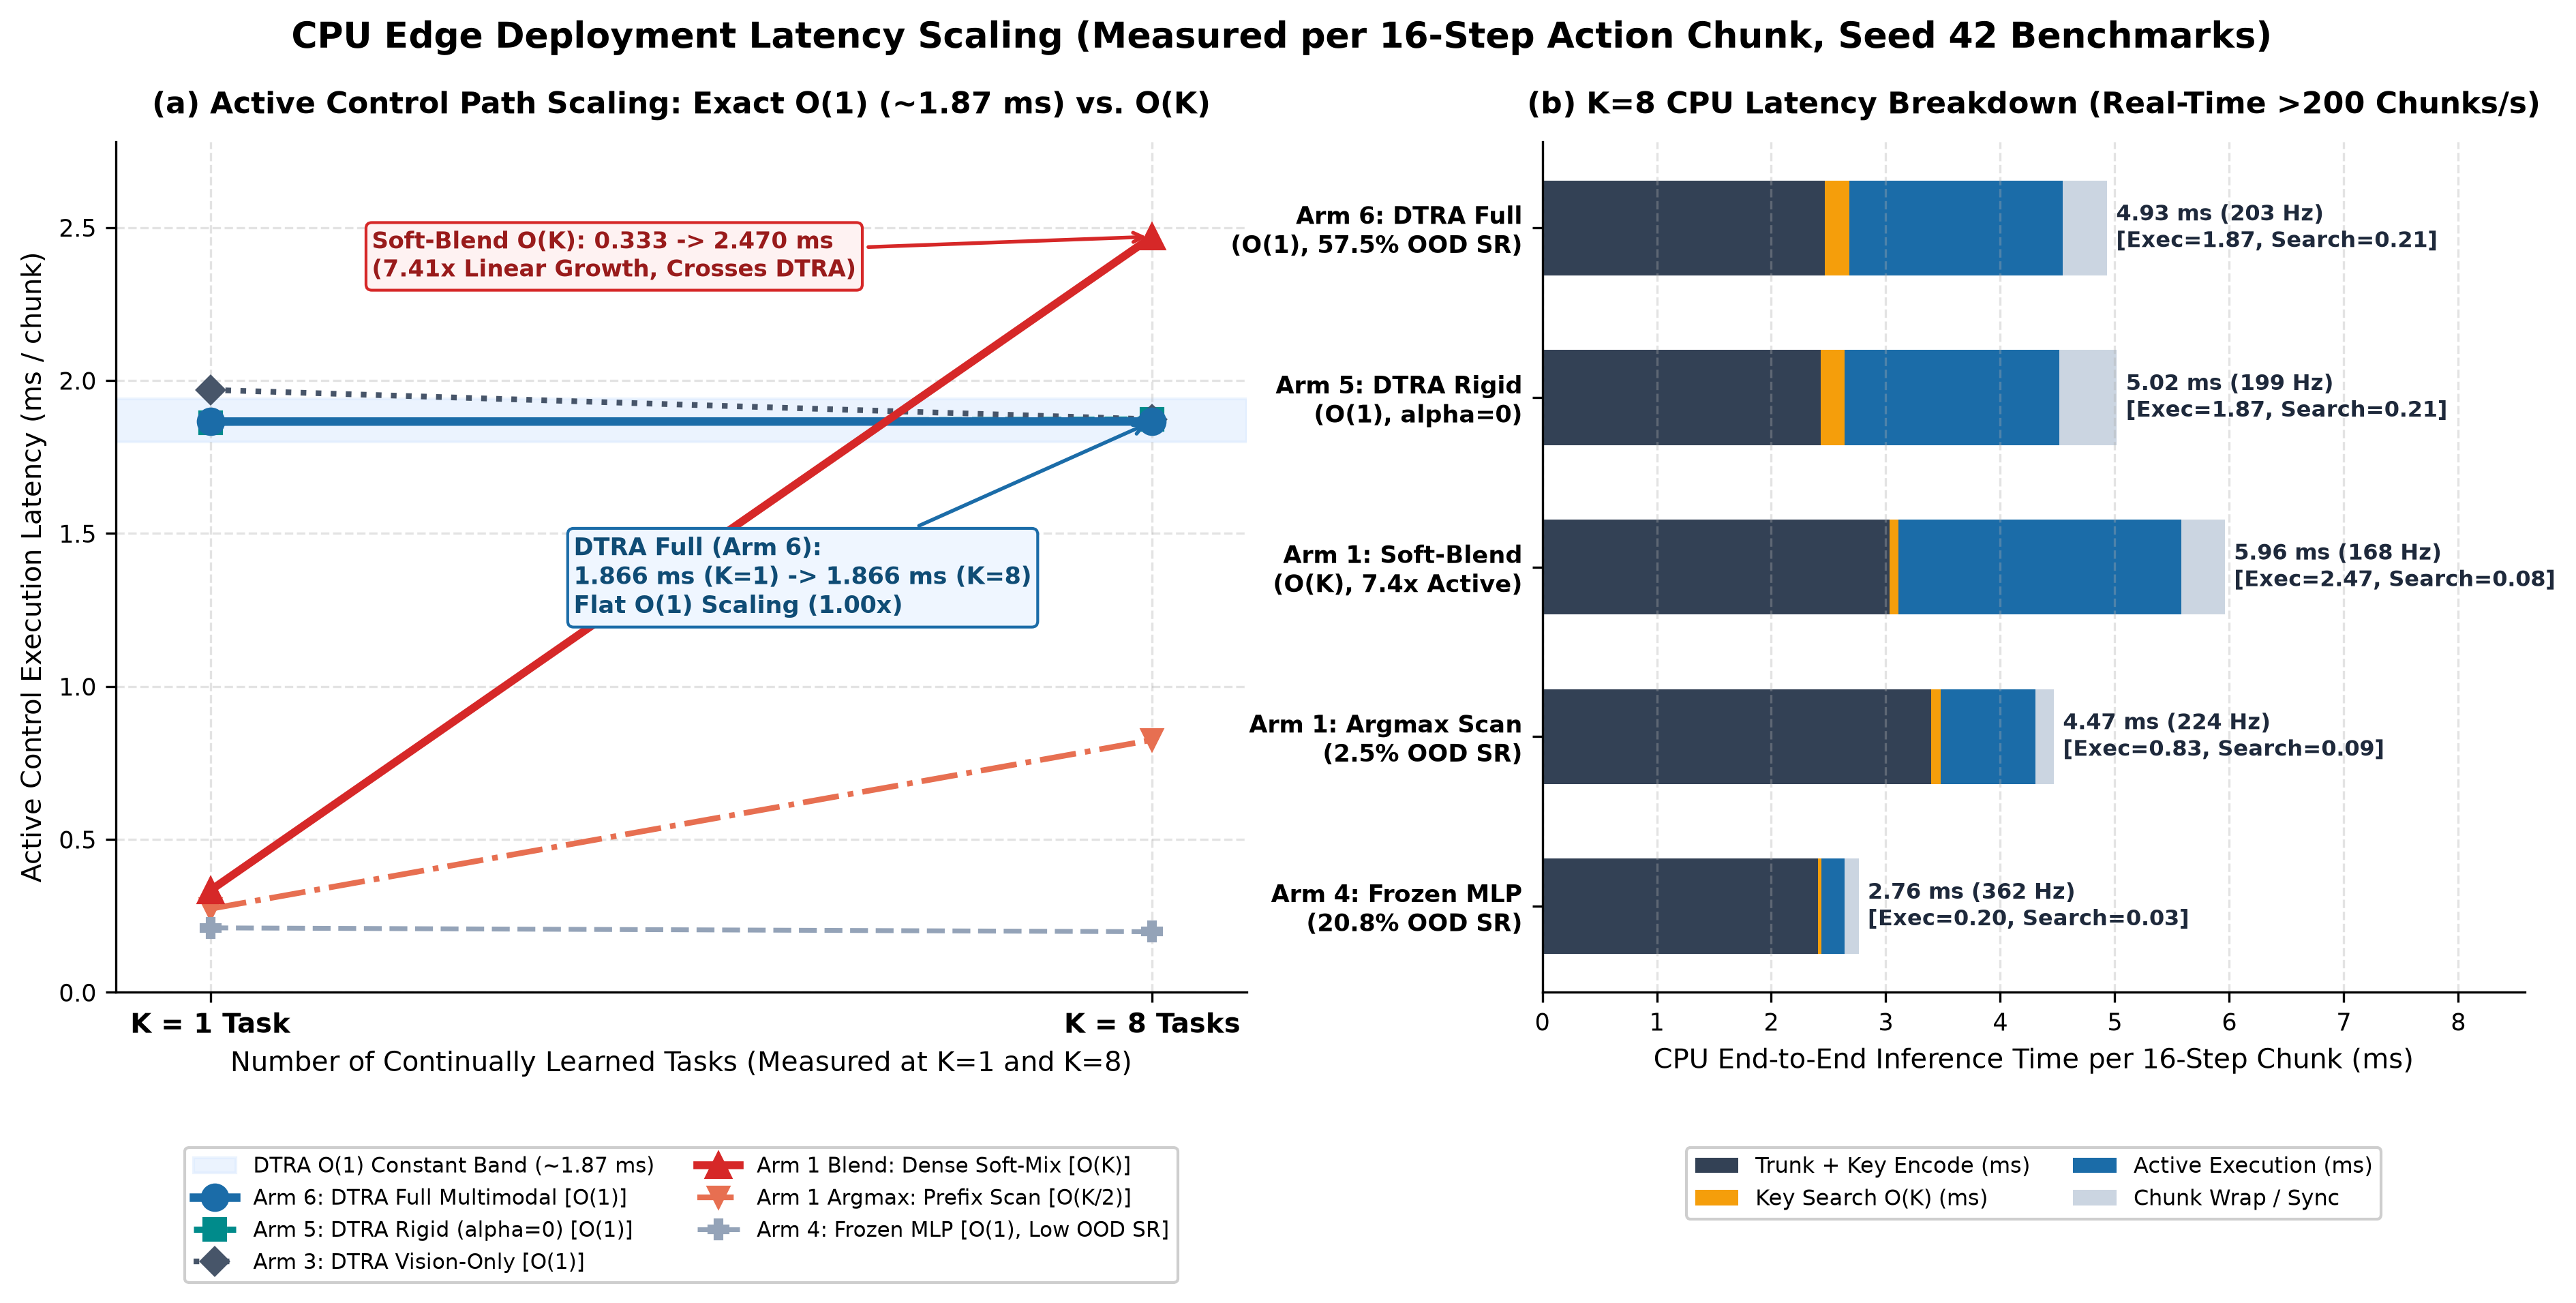
\includegraphics[width=0.82\textwidth]{../../outputs/figures/fig5_o1_latency_scaling.png}
  \caption{\textbf{Constant $O(1)$ Active Core Execution Latency vs.\ $O(K)$ Residual Chaining.} Active DTRA computation remains invariant across increasing library size ($1.87\,$ms on CPU from $K=1 \to 8$), avoiding linear latency degradation.}
  \label{fig:o1_latency}
\end{figure}


\clearpage
\section{LIBERO-100 Detailed Milestone Splits, Stratified Scenes \& Reproducibility}
\label{app:libero_details}

Table~\ref{tab:seed_registry} documents the exact provenance of every LIBERO-100 ($K=100$) JSON artifact bound to this manuscript, and Table~\ref{tab:libero100_milestones} provides the complete five-checkpoint evaluation trajectory across all parity arms and metrics. All summary tables strictly parse finalized \texttt{\_locked.json} checkpoints (full 4-arm suite on Seeds~42 \& 100 [$N=2$]; 2-arm core parity on Seeds~42, 100, and~2026 [$N=3$]).

\begin{table}[ht!]
  \centering
  \caption{Provenance and verification registry of LIBERO-100 ($K=100$) multi-seed artifacts.}
  \label{tab:seed_registry}
  \tblfont
  \setlength{\tabcolsep}{3.5pt}
  \begin{tabular}{>{\raggedright\arraybackslash}p{0.09\textwidth}>{\raggedright\arraybackslash}p{0.17\textwidth}>{\raggedright\arraybackslash}p{0.31\textwidth}>{\raggedright\arraybackslash}p{0.36\textwidth}}
    \toprule
    \textbf{Seed} & \textbf{Status} & \textbf{Completed Coverage} & \textbf{Verified Local Artifact Path} \\
    \midrule
    Seed~42 & Verified (\texttt{COMPLETED}) & 4 Arms (\texttt{arm\_\allowbreak frozen\_\allowbreak mlp, arm\_\allowbreak dtra\_\allowbreak elastic, arm\_\allowbreak dtra\_\allowbreak rigid, arm\_\allowbreak er\_\allowbreak 5pct}) & \texttt{benchmark\_\allowbreak dtra\_\allowbreak libero\_\allowbreak 10\_\allowbreak libero\_\allowbreak 90\_\allowbreak k100\_\allowbreak seed42\_\allowbreak locked.json} \\
    Seed~100 & Verified (\texttt{COMPLETED}) & 4 Arms (\texttt{arm\_\allowbreak frozen\_\allowbreak mlp, arm\_\allowbreak dtra\_\allowbreak elastic, arm\_\allowbreak dtra\_\allowbreak rigid, arm\_\allowbreak er\_\allowbreak 5pct}) & \texttt{benchmark\_\allowbreak dtra\_\allowbreak libero\_\allowbreak 10\_\allowbreak libero\_\allowbreak 90\_\allowbreak k100\_\allowbreak seed100\_\allowbreak locked.json} \\
    Seed~2026 & Verified (\texttt{COMPLETED}) & 2 Arms (\texttt{arm\_\allowbreak frozen\_\allowbreak mlp, arm\_\allowbreak dtra\_\allowbreak elastic}) & \texttt{benchmark\_\allowbreak dtra\_\allowbreak libero\_\allowbreak 10\_\allowbreak libero\_\allowbreak 90\_\allowbreak k100\_\allowbreak seed2026\_\allowbreak locked.json} \\
    \bottomrule
  \end{tabular}
\end{table}


\begin{table}[ht!]
  \centering
  \caption{Full LIBERO-100 ($K=10 \to 100$) Multi-Metric Continual Milestones under Strict Encoder Parity ($N=3$ across Seeds~[42, 100, 2026] for Frozen MLP \& DTRA Elastic; $N=2$ across Seeds~[42, 100] for ER~5\% \& DTRA Rigid).}
  \label{tab:libero100_milestones}
  \tblfont
  \setlength{\tabcolsep}{3.2pt}
  \begin{tabular}{llcccccc}
    \toprule
    \textbf{$K$} & \textbf{Arm (Strict Parity)} & \textbf{Mean SR $\uparrow$} & \textbf{FR $\downarrow$} & \textbf{BWT $\uparrow$} & \textbf{Route $\uparrow$} & \textbf{Dup-Lang $\uparrow$} & \textbf{Bases} \\
    \midrule
    $K=10$ & Frozen MLP & 82.00$\pm$4.32\% & 2.96$\pm$2.77\% & -2.96$\pm$2.77\% & 100.00$\pm$0.00\% & 100.00$\pm$0.00\% & 10 \\
     & ER 5\% (Replay) & 62.00$\pm$2.00\% & 22.22$\pm$6.67\% & -22.22$\pm$6.67\% & --- & --- & 1 \\
     & DTRA Rigid ($\alpha=0$) & 84.00$\pm$2.00\% & 2.22$\pm$0.00\% & +2.22$\pm$2.22\% & 100.00$\pm$0.00\% & 100.00$\pm$0.00\% & 7 \\
     & \textbf{DTRA Elastic (Ours)} & 80.00$\pm$1.63\% & 2.96$\pm$1.05\% & -1.48$\pm$2.77\% & 100.00$\pm$0.00\% & 100.00$\pm$0.00\% & 7 \\
    \midrule
    $K=30$ & Frozen MLP & 85.11$\pm$2.79\% & 2.99$\pm$2.28\% & -1.84$\pm$1.72\% & 96.34$\pm$0.46\% & 85.71$\pm$0.00\% & 30 \\
     & ER 5\% (Replay) & 59.67$\pm$6.33\% & 26.21$\pm$2.76\% & -24.14$\pm$4.14\% & --- & --- & 1 \\
     & DTRA Rigid ($\alpha=0$) & 90.33$\pm$1.00\% & 2.07$\pm$0.69\% & +1.38$\pm$1.38\% & 100.00$\pm$0.00\% & 100.00$\pm$0.00\% & 13 \\
     & \textbf{DTRA Elastic (Ours)} & \textbf{91.11$\pm$1.37\%} & 1.15$\pm$0.86\% & +1.84$\pm$2.28\% & \textbf{100.00$\pm$0.00\%} & \textbf{100.00$\pm$0.00\%} & 13 \\
    \midrule
    $K=50$ & Frozen MLP & 79.07$\pm$0.50\% & 2.31$\pm$2.22\% & -0.95$\pm$1.64\% & 89.04$\pm$0.75\% & 61.54$\pm$1.82\% & 50 \\
     & ER 5\% (Replay) & 54.80$\pm$2.40\% & 25.51$\pm$0.20\% & -21.22$\pm$1.22\% & --- & --- & 1 \\
     & DTRA Rigid ($\alpha=0$) & 91.00$\pm$1.00\% & 2.04$\pm$0.41\% & +1.22$\pm$0.41\% & 100.00$\pm$0.00\% & 100.00$\pm$0.00\% & 22 \\
     & \textbf{DTRA Elastic (Ours)} & \textbf{90.67$\pm$1.00\%} & 2.45$\pm$1.00\% & +0.54$\pm$1.26\% & \textbf{100.00$\pm$0.00\%} & \textbf{100.00$\pm$0.00\%} & 22 \\
    \midrule
    $K=70$ & Frozen MLP & 76.48$\pm$0.97\% & 3.19$\pm$1.44\% & -0.19$\pm$2.39\% & 87.96$\pm$0.91\% & 58.57$\pm$4.10\% & 70 \\
     & ER 5\% (Replay) & 49.14$\pm$4.00\% & 28.84$\pm$1.30\% & -23.62$\pm$3.04\% & --- & --- & 1 \\
     & DTRA Rigid ($\alpha=0$) & 87.14$\pm$0.57\% & 3.33$\pm$0.72\% & -0.14$\pm$0.43\% & 100.00$\pm$0.00\% & 100.00$\pm$0.00\% & 24 \\
     & \textbf{DTRA Elastic (Ours)} & \textbf{87.71$\pm$0.70\%} & 2.42$\pm$0.27\% & +0.68$\pm$0.36\% & \textbf{100.00$\pm$0.00\%} & \textbf{100.00$\pm$0.00\%} & 24 \\
    \midrule
    $K=100$ & Frozen MLP & 70.33$\pm$1.18\% & 2.90$\pm$1.05\% & +0.20$\pm$2.29\% & 81.94$\pm$0.24\% & 41.76$\pm$2.09\% & 100 \\
     & ER 5\% (Replay) & 40.50$\pm$0.30\% & 27.07$\pm$4.04\% & -20.71$\pm$2.93\% & --- & --- & 1 \\
     & DTRA Rigid ($\alpha=0$) & 86.20$\pm$0.00\% & 2.93$\pm$0.91\% & +0.10$\pm$0.91\% & 99.86$\pm$0.14\% & 99.53$\pm$0.47\% & 27 \\
     & \textbf{DTRA Elastic (Ours)} & \textbf{87.00$\pm$0.86\%} & 2.69$\pm$0.67\% & +0.20$\pm$0.72\% & \textbf{99.90$\pm$0.13\%} & \textbf{99.68$\pm$0.45\%} & 27 \\
    \bottomrule
  \end{tabular}
\end{table}



\begin{table}[ht!]
  \centering
  \caption{LIBERO-Goal 5-Task 7-DoF Pilot Benchmark (Seed~42, $n_{\text{eval}}=5$, Peak VRAM $\le 3.7$\,GB).}
  \label{tab:libero_goal_pilot}
  \small
  \setlength{\tabcolsep}{5pt}
  \begin{tabular}{lccccc}
    \toprule
    \textbf{Method (4 Parity Arms)} & \textbf{Mean SR $\uparrow$} & \textbf{FR $\downarrow$} & \textbf{BWT $\uparrow$} & \textbf{Route $\uparrow$} & \textbf{Peak VRAM} \\
    \midrule
    Frozen Slot MLP (Baseline) & 100.0\% & 0.0\% & +15.0\% & 100.0\% & 3695\,MB \\
    Experience Replay (5\%) & 88.0\% & 10.0\% & -5.0\% & --- & 3298\,MB \\
    DTRA Rigid ($\alpha=0$) & 88.0\% & 10.0\% & -5.0\% & 100.0\% & 3696\,MB \\
    \textbf{DTRA Elastic (Ours)} & 92.0\% & 5.0\% & +0.0\% & 100.0\% & 3696\,MB \\
    \bottomrule
  \end{tabular}
\end{table}


\clearpage
\subsection{Long-Horizon (\texttt{libero\_10}) vs.\ High-Density (\texttt{libero\_90}) Crossover Split}
Splitting the 100-task continual stream at $K=100$ exposes the density-driven crossover inside one curriculum (Table~\ref{tab:libero_split}). On the initial 10 long-horizon tasks (\texttt{libero\_10}), unconstrained MLPs memorize sparse skills cleanly, whereas across the high-density 90-task suffix (\texttt{libero\_90}), DTRA sustains near-perfect routing and lifts Success Rate dramatically. Table~\ref{tab:libero_resources} reports Forward Transfer (FWT), parameter footprint, peak VRAM, and GPU active latency.

\begin{table}[ht!]
  \centering
  \caption{LIBERO-100 Final $K=100$ Suite Split: Initial 10 Long-Horizon Tasks vs.\ High-Density 90-Task Suffix ($N=3$ across Seeds~[42, 100, 2026] for Frozen MLP \& DTRA Elastic; $N=2$ across Seeds~[42, 100] for ER~5\% \& DTRA Rigid).}
  \label{tab:libero_split}
  \tblfont
  \setlength{\tabcolsep}{3.0pt}
  \begin{tabular}{lccccc}
    \toprule
    \textbf{Method} & \textbf{\texttt{libero\_10} SR} & \textbf{\texttt{libero\_10} Route} & \textbf{\texttt{libero\_90} SR} & \textbf{\texttt{libero\_90} Route} & \textbf{$\Delta$ (\texttt{L90}$-$\texttt{L10})} \\
    \midrule
    Frozen MLP & 86.00$\pm$4.32\% & 100.00$\pm$0.00\% & 68.59$\pm$1.03\% & 79.93$\pm$0.26\% & -17.41\%p \\
    ER 5\% & 31.00$\pm$3.00\% & --- & 41.56$\pm$0.67\% & --- & +10.56\%p \\
    DTRA Rigid ($\alpha=0$) & 84.00$\pm$0.00\% & 100.00$\pm$0.00\% & 86.44$\pm$0.00\% & 99.84$\pm$0.16\% & +2.44\%p \\
    \textbf{DTRA Elastic} & 81.33$\pm$2.49\% & 100.00$\pm$0.00\% & 87.63$\pm$0.69\% & 99.89$\pm$0.15\% & +6.30\%p \\
    \bottomrule
  \end{tabular}
\end{table}

\begin{table}[ht!]
  \centering
  \caption{LIBERO-100 Resource Footprint, Forward Transfer (FWT), Peak VRAM, and GPU Control Latency at $K=100$ ($N=3$ for Frozen MLP \& DTRA Elastic; $N=2$ for ER~5\% \& DTRA Rigid).}
  \label{tab:libero_resources}
  \tblfont
  \setlength{\tabcolsep}{4.2pt}
  \begin{tabular}{lcccc}
    \toprule
    \textbf{Method} & \textbf{FWT $\uparrow$} & \textbf{Total Params (MB)} & \textbf{Peak CUDA VRAM} & \textbf{Active Latency} \\
    \midrule
    Frozen MLP & -9.97$\pm$17.34\% & 151.67$\pm$0.00\,MB & 2602$\pm$0\,MB & 6.46$\pm$0.57\,ms \\
    ER 5\% & -19.19$\pm$2.63\% & 1.70$\pm$0.00\,MB & 4772$\pm$0\,MB & 5.34$\pm$0.03\,ms \\
    DTRA Rigid ($\alpha=0$) & +6.16$\pm$0.91\% & 183.14$\pm$0.00\,MB & 2800$\pm$0\,MB & 9.36$\pm$0.05\,ms \\
    \textbf{DTRA Elastic} & +0.13$\pm$9.24\% & 183.14$\pm$0.00\,MB & 2713$\pm$77\,MB & 9.55$\pm$0.20\,ms \\
    \bottomrule
  \end{tabular}
\end{table}

The reported $73\%$ reduction refers to the number of shared primitive bases relative to one basis per task, rather than a reduction in total parameter memory.

\begin{table}[ht!]
  \centering
  \caption{Strict-Parity Experimental Protocol \& Architectural Hyperparameter Schedule (LIBERO-100 \& Meta-World).}
  \label{tab:hyperparams}
  \tblfont
  \setlength{\tabcolsep}{3.8pt}
  \begin{tabular}{>{\raggedright\arraybackslash}p{0.145\textwidth}>{\raggedright\arraybackslash}p{0.265\textwidth}>{\raggedright\arraybackslash}p{0.295\textwidth}>{\raggedright\arraybackslash}p{0.215\textwidth}}
    \toprule
    \textbf{Subsystem} & \textbf{Parameter / Mechanism} & \textbf{LIBERO-100 Value} & \textbf{Meta-World v3 Value} \\
    \midrule
    Optimizer & AdamW lr / decay / batch / ep. & \texttt{5e-4} / excl. frozen / 128 / 25 & \texttt{1e-3} / 0.0 / 64 / 30 \\
    Memory Staging & Task streaming (\texttt{--stream-tasks}) & On-demand HDF5 ($\le 2.8$\,GB VRAM) & Single-session cache \\
    Perception & Backbone + grids + DoG + Text & ResNet-18 ($4\times 4,2\times 2$)+DoG+Hash & ResNet-18 + DoG + Hash \\
    Manifold Key & $d_{\text{key}}$ / Hypersphere proj. & $128 \to \mathbb{S}^{63}$ orthogonal $P_{\text{topo}}$ & $128 \to \mathbb{S}^{63}$ orthogonal \\
    Action Chunk & Clamped $C^2$ cubic B-Spline & $N_k=6$ bases ($8$ reg.) $\to H=16$, exec~$8$ & $N_k=6 \to H=16$, exec~$8$ \\
    Anti-Encroach. & Constraint + Stage-2 Top-$M$ CMC & Cache $\mu_j, s_{jj}$; $M=5$, $\gamma_{\text{cm}}=1.0$ & Contrastive margin $\tau_i$ \\
    Basis \& Reset & SharedBasisBank + 2-Timescale & $K=100 \to 27$ frozen; snap $0.0000$ & 8 cells; snap $0.0000$ \\
    Evaluation & Rollouts ($n_{\text{eval}}$) / Checkpoints & $5$ / $K \in \{10,30,50,70,100\}$ & $15$ clean / $8$ severe OOD \\
    \bottomrule
  \end{tabular}
\end{table}

\clearpage
\subsection{Duplicate-Language Stratification, Scene Groups \& Per-Task \texttt{libero\_10} Profile}
To verify that gains are uniform across kitchen, living-room, and study manipulation environments rather than confined to a single scene, Table~\ref{tab:libero_stratified} disaggregates final $K=100$ evaluation vectors into Duplicate-Instruction tasks ($30$ tasks across $13$ ambiguous instruction groups), Unique-Instruction tasks ($70$ tasks), and the three \texttt{libero\_90} scene domains. Table~\ref{tab:libero10_pertask} reports individual long-horizon \texttt{libero\_10} task outcomes (\texttt{T00}--\texttt{T09}) alongside chunk counts and B-Spline reconstruction RMSE.

\begin{table}[ht!]
  \centering
  \caption{LIBERO-100 ($K=100$) Stratified Final Mean SR (and Routing Accuracy) by Instruction Ambiguity \& \texttt{libero\_90} Scene Domain ($N=3$ for Frozen MLP \& DTRA Elastic; $N=2$ for ER~5\% \& DTRA Rigid).}
  \label{tab:libero_stratified}
  \tblfont
  \setlength{\tabcolsep}{2.4pt}
  \begin{tabular}{lccccc}
    \toprule
    \textbf{Method} & \textbf{Dup-Lang (30)} & \textbf{Unique-Lang (70)} & \textbf{Kitchen (L90)} & \textbf{Living Rm (L90)} & \textbf{Study (L90)} \\
    \midrule
    Frozen MLP & 35.8$\pm$0.3\% (41.8$\pm$2.1\%) & 85.1$\pm$1.6\% (99.2$\pm$0.6\%) & 79.0$\pm$0.5\% & 69.6$\pm$3.2\% & 38.8$\pm$1.9\% \\
    ER 5\% & 36.3$\pm$2.3\% (---) & 42.3$\pm$0.6\% (---) & 51.1$\pm$0.2\% & 44.1$\pm$3.3\% & 11.8$\pm$2.4\% \\
    DTRA Rigid ($\alpha=0$) & 88.0$\pm$0.7\% (99.5$\pm$0.5\%) & 85.4$\pm$0.3\% (100.0$\pm$0.0\%) & 93.0$\pm$0.0\% & 74.4$\pm$1.1\% & 87.6$\pm$1.8\% \\
    \textbf{DTRA Elastic} & 90.7$\pm$1.4\% (99.7$\pm$0.4\%) & 85.4$\pm$0.7\% (100.0$\pm$0.0\%) & 93.5$\pm$0.7\% & 75.6$\pm$1.0\% & 91.0$\pm$3.6\% \\
    \bottomrule
  \end{tabular}
\end{table}

\begin{table}[ht!]
  \centering
  \caption{Individual Long-Horizon \texttt{libero\_10} Task Breakdown (\texttt{T00}--\texttt{T09}): Chunks, $C^2$ B-Spline RMSE, and $K=100$ Final SR (\%, $N=3$ for Frozen MLP \& DTRA Elastic; $N=2$ for DTRA Rigid).}
  \label{tab:libero10_pertask}
  \tblfont
  \setlength{\tabcolsep}{2.6pt}
  \begin{tabular}{l>{\raggedright\arraybackslash}p{0.33\textwidth}ccccc}
    \toprule
    \textbf{ID} & \textbf{LIBERO-10 Task Identifier} & \textbf{Ch.} & \textbf{RMSE} & \textbf{Frozen MLP} & \textbf{DTRA Rigid} & \textbf{DTRA Elastic} \\
    \midrule
    \texttt{T00} & \texttt{LR\_S2\_put\_both\_the\_alphabet\_soup\_...} & 14600 & 0.0479 & 80.0$\pm$16.3\% & 80.0$\pm$0.0\% & \textbf{66.7$\pm$9.4\%} \\
    \texttt{T01} & \texttt{LR\_S2\_put\_both\_the\_cream\_cheese\_b...} & 12921 & 0.0504 & 73.3$\pm$9.4\% & 80.0$\pm$0.0\% & \textbf{80.0$\pm$0.0\%} \\
    \texttt{T02} & \texttt{KT\_S3\_turn\_on\_the\_stove\_and\_put\_t...} & 13198 & 0.0490 & 100.0$\pm$0.0\% & 100.0$\pm$0.0\% & \textbf{100.0$\pm$0.0\%} \\
    \texttt{T03} & \texttt{KT\_S4\_put\_the\_black\_bowl\_in\_the\_b...} & 12334 & 0.0360 & 100.0$\pm$0.0\% & 90.0$\pm$10.0\% & \textbf{93.3$\pm$9.4\%} \\
    \texttt{T04} & \texttt{LR\_S5\_put\_the\_white\_mug\_on\_the\_le...} & 12809 & 0.0501 & 86.7$\pm$9.4\% & 90.0$\pm$10.0\% & \textbf{86.7$\pm$9.4\%} \\
    \texttt{T05} & \texttt{ST\_S1\_pick\_up\_the\_book\_and\_place\_...} & 9370 & 0.0311 & 80.0$\pm$0.0\% & 100.0$\pm$0.0\% & \textbf{100.0$\pm$0.0\%} \\
    \texttt{T06} & \texttt{LR\_S6\_put\_the\_white\_mug\_on\_the\_pl...} & 12656 & 0.0485 & 60.0$\pm$16.3\% & 50.0$\pm$10.0\% & \textbf{40.0$\pm$0.0\%} \\
    \texttt{T07} & \texttt{LR\_S1\_put\_both\_the\_alphabet\_soup\_...} & 13376 & 0.0494 & 80.0$\pm$16.3\% & 100.0$\pm$0.0\% & \textbf{86.7$\pm$9.4\%} \\
    \texttt{T08} & \texttt{KT\_S8\_put\_both\_moka\_pots\_on\_the\_s...} & 20694 & 0.0391 & 100.0$\pm$0.0\% & 50.0$\pm$10.0\% & \textbf{73.3$\pm$24.9\%} \\
    \texttt{T09} & \texttt{KT\_S6\_put\_the\_yellow\_and\_white\_mu...} & 15132 & 0.0345 & 100.0$\pm$0.0\% & 100.0$\pm$0.0\% & \textbf{86.7$\pm$9.4\%} \\
    \bottomrule
  \end{tabular}
\end{table}

\clearpage
\section{3D Meta-World Detailed Per-Task Analysis \& 9-Regime OOD Curves}
\label{app:metaworld_details}

Table~\ref{tab:mw_pertask} reports per-task Clean vs.\ Severe Gaussian OOD ($\sigma=0.20$) success rates averaged across all 3 seeds (42, 100, 2026) over the 8 sequential Meta-World v3 manipulation tasks, while Table~\ref{tab:mw_supp} summarizes Seed~42 traditional continual learning baselines (Naive FT, EWC, ER~5\%) alongside reverse task ordering ($T_7 \to T_0$) invariance. Table~\ref{tab:mw_ood9} details the 9-regime visual perturbation curves measured in \texttt{ablate\_dtra\_supplemental\_results.json}, Table~\ref{tab:mw_snapback} verifies post-episode buffer reset to exact $0.0000$, and Figure~\ref{fig:mw_cl_heatmap} compares the $8\times 8$ continual retention matrices.

\begin{table}[ht!]
  \centering
  \caption{3D Meta-World 8-Task 3-Seed Mean Clean / Severe OOD ($\sigma=0.20$) Success Rates (\%) per Task.}
  \label{tab:mw_pertask}
  \tblfont
  \setlength{\tabcolsep}{2.8pt}
  \begin{tabular}{lcccc}
    \toprule
    \textbf{Meta-World Task ($T_0 \to T_7$)} & \textbf{ABK-VLA DoG} & \textbf{Frozen MLP (MM)} & \textbf{DTRA Rigid} & \textbf{DTRA Full (MM)} \\
    \midrule
    \texttt{button-press-v3} & 95.6 / 2.2 & 84.4 / 40.0 & 93.3 / 53.3 & \textbf{93.3 / 62.2} \\
    \texttt{door-open-v3} & 86.7 / 0.0 & 71.1 / 0.0 & 86.7 / 33.3 & \textbf{57.8 / 46.7} \\
    \texttt{window-open-v3} & 68.9 / 0.0 & 62.2 / 0.0 & 44.4 / 35.6 & \textbf{37.8 / 31.1} \\
    \texttt{faucet-open-v3} & 97.8 / 0.0 & 100.0 / 0.0 & 88.9 / 48.9 & \textbf{95.6 / 71.1} \\
    \texttt{drawer-open-v3} & 64.4 / 0.0 & 91.1 / 0.0 & 71.1 / 51.1 & \textbf{66.7 / 35.6} \\
    \texttt{drawer-close-v3} & 93.3 / 6.7 & 93.3 / 57.8 & 100.0 / 93.3 & \textbf{100.0 / 53.3} \\
    \texttt{handle-press-v3} & 97.8 / 0.0 & 91.1 / 68.9 & 68.9 / 62.2 & \textbf{73.3 / 64.4} \\
    \texttt{coffee-button-v3} & 57.8 / 8.9 & 91.1 / 22.2 & 68.9 / 51.1 & \textbf{53.3 / 46.7} \\
    \bottomrule
  \end{tabular}
\end{table}


\begin{table}[ht!]
  \centering
  \caption{Supplemental 3D Meta-World Baselines (Seed~42) and Reverse Task Ordering ($T_7 \to T_0$) Order-Invariance Verification.}
  \label{tab:mw_supp}
  \tblfont
  \setlength{\tabcolsep}{6pt}
  \begin{tabular}{lccc}
    \toprule
    \textbf{Method / Ordering} & \textbf{Clean SR $\uparrow$} & \textbf{FR $\downarrow$} & \textbf{Severe OOD SR $\uparrow$} \\
    \midrule
    Naive Fine-Tuning (Seed 42) & 12.5\% & 98.1\% & 5.8\% \\
    EWC ($\lambda=500$, Seed 42) & 11.7\% & 100.0\% & 18.3\% \\
    Experience Replay (5\%, Seed 42) & 77.5\% & 20.0\% & 25.0\% \\
    \textbf{DTRA Reverse ($T_7 \to T_0$, Ours)} & \textbf{74.2\%} & \textbf{0.0\%} & \textbf{64.2\%} \\
    \bottomrule
  \end{tabular}
\end{table}


\clearpage
\begin{table}[ht!]
  \centering
  \caption{9-Regime Zero-Shot Visual OOD Stress Evaluation (Seed~42, Mean SR\% and Routing Accuracy in Parentheses).}
  \label{tab:mw_ood9}
  \tblfont
  \setlength{\tabcolsep}{2.8pt}
  \begin{tabular}{lcccc}
    \toprule
    \textbf{Perturbation Regime} & \textbf{DTRA Vision} & \textbf{Frozen MLP} & \textbf{DTRA Rigid} & \textbf{DTRA Full (MM)} \\
    \midrule
    Clean Nominal (No Perturb.) & 73.3\% (99\%) & 90.8\% (100\%) & 73.3\% (100\%) & \textbf{81.7\% (100\%)} \\
    Gaussian Noise ($\sigma=0.05$) & 71.7\% (99\%) & 56.7\% (100\%) & 71.7\% (100\%) & \textbf{73.3\% (100\%)} \\
    Gaussian Noise ($\sigma=0.10$) & 59.2\% (97\%) & 37.5\% (100\%) & 64.2\% (100\%) & \textbf{63.3\% (100\%)} \\
    Gaussian Noise ($\sigma=0.20$) & 45.8\% (93\%) & 32.5\% (100\%) & 55.8\% (100\%) & \textbf{50.8\% (100\%)} \\
    Severe Gaussian ($\sigma=0.30$) & 38.3\% (88\%) & 34.2\% (100\%) & 58.3\% (100\%) & \textbf{50.8\% (100\%)} \\
    Spatial Cutout ($15\%$) & 21.7\% (36\%) & 33.3\% (100\%) & 55.8\% (100\%) & \textbf{51.7\% (100\%)} \\
    Severe Cutout ($30\%$) & 9.2\% (20\%) & 35.8\% (100\%) & 46.7\% (100\%) & \textbf{46.7\% (100\%)} \\
    High Brightness Shift & 70.8\% (98\%) & 27.5\% (100\%) & 75.0\% (100\%) & \textbf{68.3\% (100\%)} \\
    Harsh Contrast Distortion & 75.0\% (98\%) & 74.2\% (100\%) & 74.2\% (100\%) & \textbf{79.2\% (100\%)} \\
    \bottomrule
  \end{tabular}
\end{table}

\begin{table}[ht!]
  \centering
  \caption{Two-Timescale Snap-Back Ephemeral Deformation Telemetry (Seed~42): Active compliance adapts cleanly during rollouts before resetting to exact $0.0000$.}
  \label{tab:mw_snapback}
  \tblfont
  \setlength{\tabcolsep}{4.2pt}
  \begin{tabular}{lcccc}
    \toprule
    \textbf{Regime} & \textbf{Mean $\|\Delta\mathbf{z}^*\|_2$} & \textbf{Max $\|\Delta\mathbf{z}^*\|_2$} & \textbf{Coarse / Fine Mean} & \textbf{Post-Snap Abs Max} \\
    \midrule
    Meta-World Clean Nominal (Seed~42) & 0.1649 & 0.3277 & 0.2956 / 0.0389 & \textbf{0.0000} \\
    Meta-World Severe OOD $\sigma=0.20$ (Seed~42) & 0.1697 & 0.3399 & 0.2997 / 0.0460 & \textbf{0.0000} \\
    \bottomrule
  \end{tabular}
\end{table}

\begin{figure}[ht!]
  \centering
  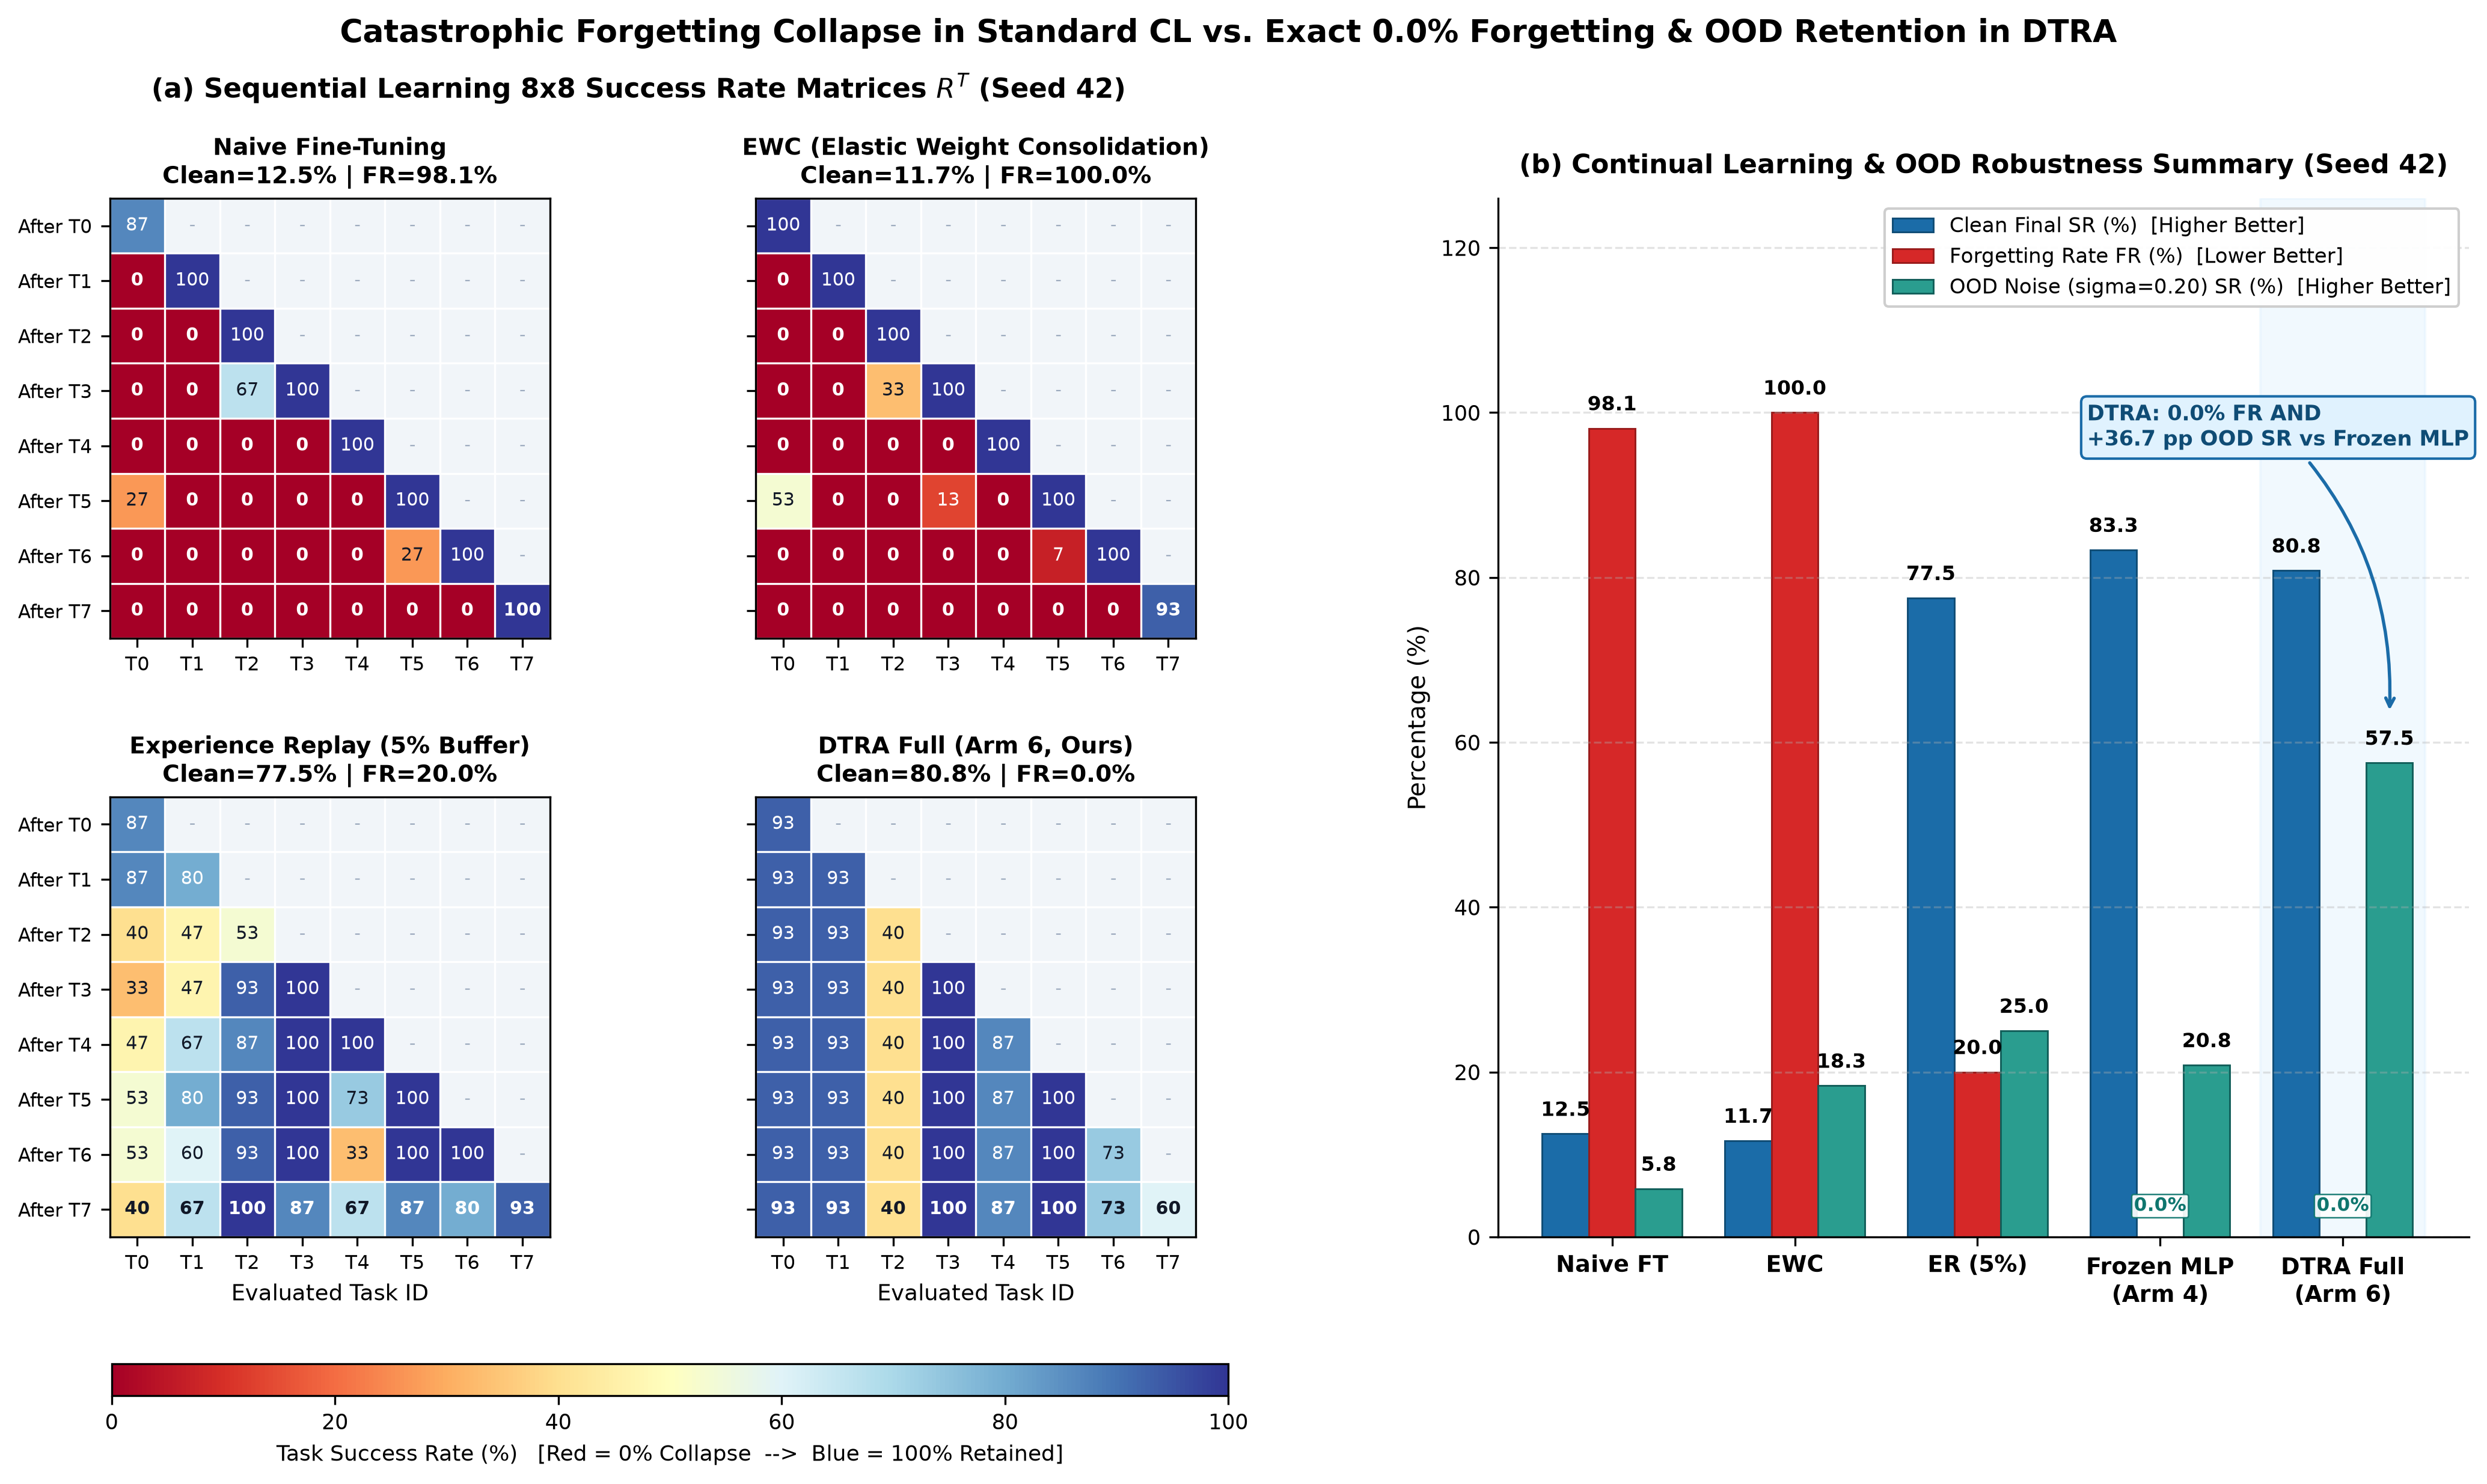
\includegraphics[width=0.76\textwidth]{../../outputs/figures/fig4_cl_forgetting_heatmap_and_bars.png}
  \caption{\textbf{8$\times$8 Continual Retention Heatmaps \& Forgetting Summary on Meta-World (Seed~42).} Shared-backbone Naive FT, EWC, and ER~5\% lose earlier tasks sequentially, whereas DTRA preserves $0.0\%$ forgetting and $100.0\%$ autonomous routing.}
  \label{fig:mw_cl_heatmap}
\end{figure}

\clearpage
\section{White-Box Routing Call Stack Logs \& 27-Basis SharedBasisBank Visualization}
\label{app:whitebox_viz}

Figure~\ref{fig:libero_basis_diag} visualizes the empirical \texttt{SharedBasisBank} saturation ($K=100 \to 27$ frozen bases, $-73\%$) and No-Encroachment key projection across all $100$ LIBERO tasks (Seed~42 \texttt{\_locked.json}), while Figure~\ref{fig:xai_rollout} presents multi-task closed-loop XAI rollout telemetry. Table~\ref{tab:callstack_log} displays 12 representative registration and post-snapback audit records parsed directly from \texttt{arm\_dtra\_elastic}, spanning \texttt{L10} and all three \texttt{L90} scene domains as well as both \texttt{Dup-Lang} and unique instructions.

\begin{figure}[ht!]
  \centering
  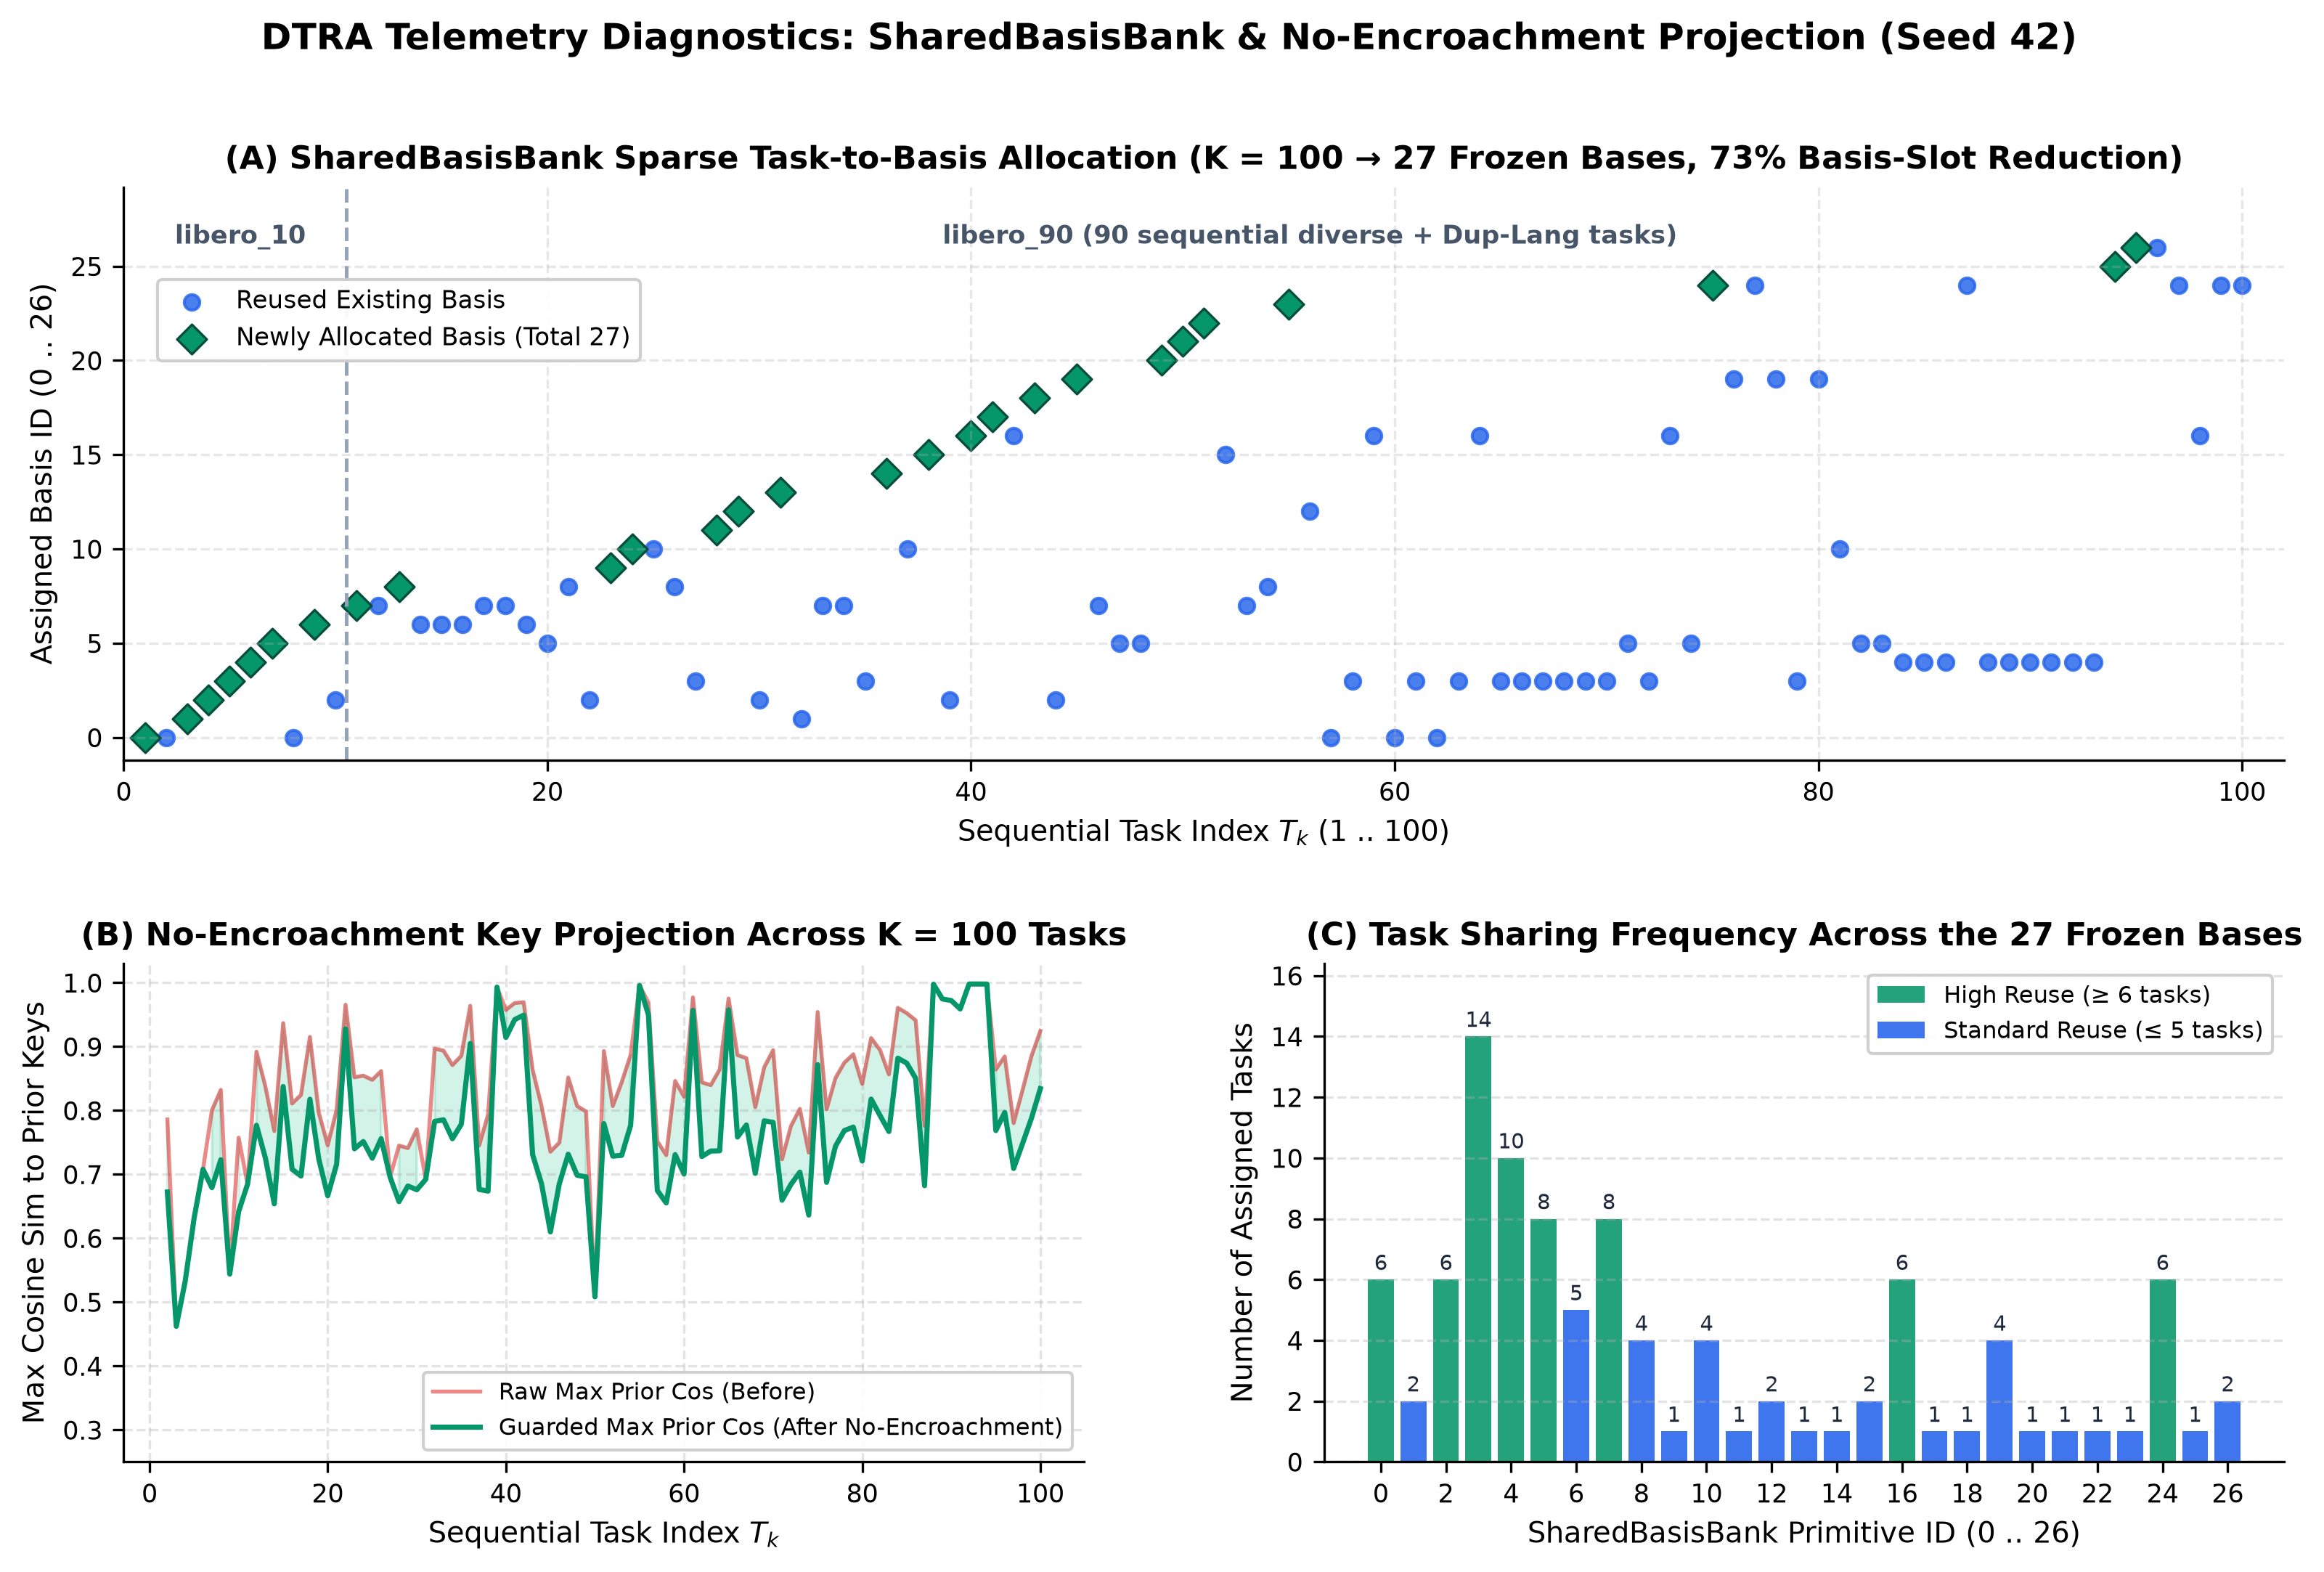
\includegraphics[width=0.84\textwidth]{../../outputs/figures/fig8_libero100_basis_and_callstack.png}
  \caption{\textbf{SharedBasisBank Allocation \& No-Encroachment Diagnostics across $K=100$ LIBERO Tasks (Seed~42).} \textbf{(A)} Sub-linear basis growth ($K=100 \to 27$, $-73\%$). \textbf{(B)} No-Encroachment orthogonal projection systematically suppresses neighbor cosine peaks. \textbf{(C)} Sharing frequency across the 27 frozen primitives.}
  \label{fig:libero_basis_diag}
\end{figure}

\begin{table}[ht!]
  \centering
  \caption{Verified White-Box Routing \& Consolidation Audit Records Parsed from \texttt{arm\_dtra\_elastic} (Seed~42 \texttt{\_locked.json}).}
  \label{tab:callstack_log}
  \tblfont
  \setlength{\tabcolsep}{4.0pt}
  \begin{tabular}{llccc}
    \toprule
    \textbf{Task (Suite/Scene/Lang)} & \textbf{Basis Slot} & \textbf{No-Enc.\ (Bef $\to$ Aft)} & \textbf{Self-Sim $s_{kk}$} & \textbf{Post-Snap} \\
    \midrule
    \texttt{T00} (L10/LIV/Unq) & \texttt{Basis\#00} (NEW) & 0.0000 $\to$ 0.0000 & 1.0000 & \textbf{0.0000} \\
    \texttt{T02} (L10/KIT/Unq) & \texttt{Basis\#01} (NEW) & 0.4621 $\to$ 0.4621 & 1.0000 & \textbf{0.0000} \\
    \texttt{T05} (L10/STU/Dup) & \texttt{Basis\#04} (NEW) & 0.7079 $\to$ 0.7079 & 1.0000 & \textbf{0.0000} \\
    \texttt{T09} (L10/KIT/Unq) & \texttt{Basis\#02} (REUSE) & 0.7575 $\to$ 0.6418 & 0.9805 & \textbf{0.0000} \\
    \texttt{T10} (L90/KIT/Dup) & \texttt{Basis\#07} (NEW) & 0.6846 $\to$ 0.6846 & 1.0000 & \textbf{0.0000} \\
    \texttt{T25} (L90/KIT/Unq) & \texttt{Basis\#08} (REUSE) & 0.8617 $\to$ 0.7560 & 0.9712 & \textbf{0.0000} \\
    \texttt{T49} (L90/KIT/Unq) & \texttt{Basis\#21} (NEW) & 0.5083 $\to$ 0.5083 & 1.0000 & \textbf{0.0000} \\
    \texttt{T64} (L90/LIV/Dup) & \texttt{Basis\#03} (REUSE) & 0.9753 $\to$ 0.9574 & 0.9940 & \textbf{0.0000} \\
    \texttt{T79} (L90/LIV/Unq) & \texttt{Basis\#19} (REUSE) & 0.8416 $\to$ 0.7209 & 0.9738 & \textbf{0.0000} \\
    \texttt{T88} (L90/STU/Dup) & \texttt{Basis\#04} (REUSE) & 0.9746 $\to$ 0.9746 & 1.0000 & \textbf{0.0000} \\
    \texttt{T95} (L90/STU/Unq) & \texttt{Basis\#26} (REUSE) & 0.8846 $\to$ 0.7970 & 0.9634 & \textbf{0.0000} \\
    \texttt{T99} (L90/STU/Unq) & \texttt{Basis\#24} (REUSE) & 0.9247 $\to$ 0.8342 & 0.9735 & \textbf{0.0000} \\
    \bottomrule
  \end{tabular}
\end{table}

\clearpage
\begin{figure}[ht!]
  \centering
  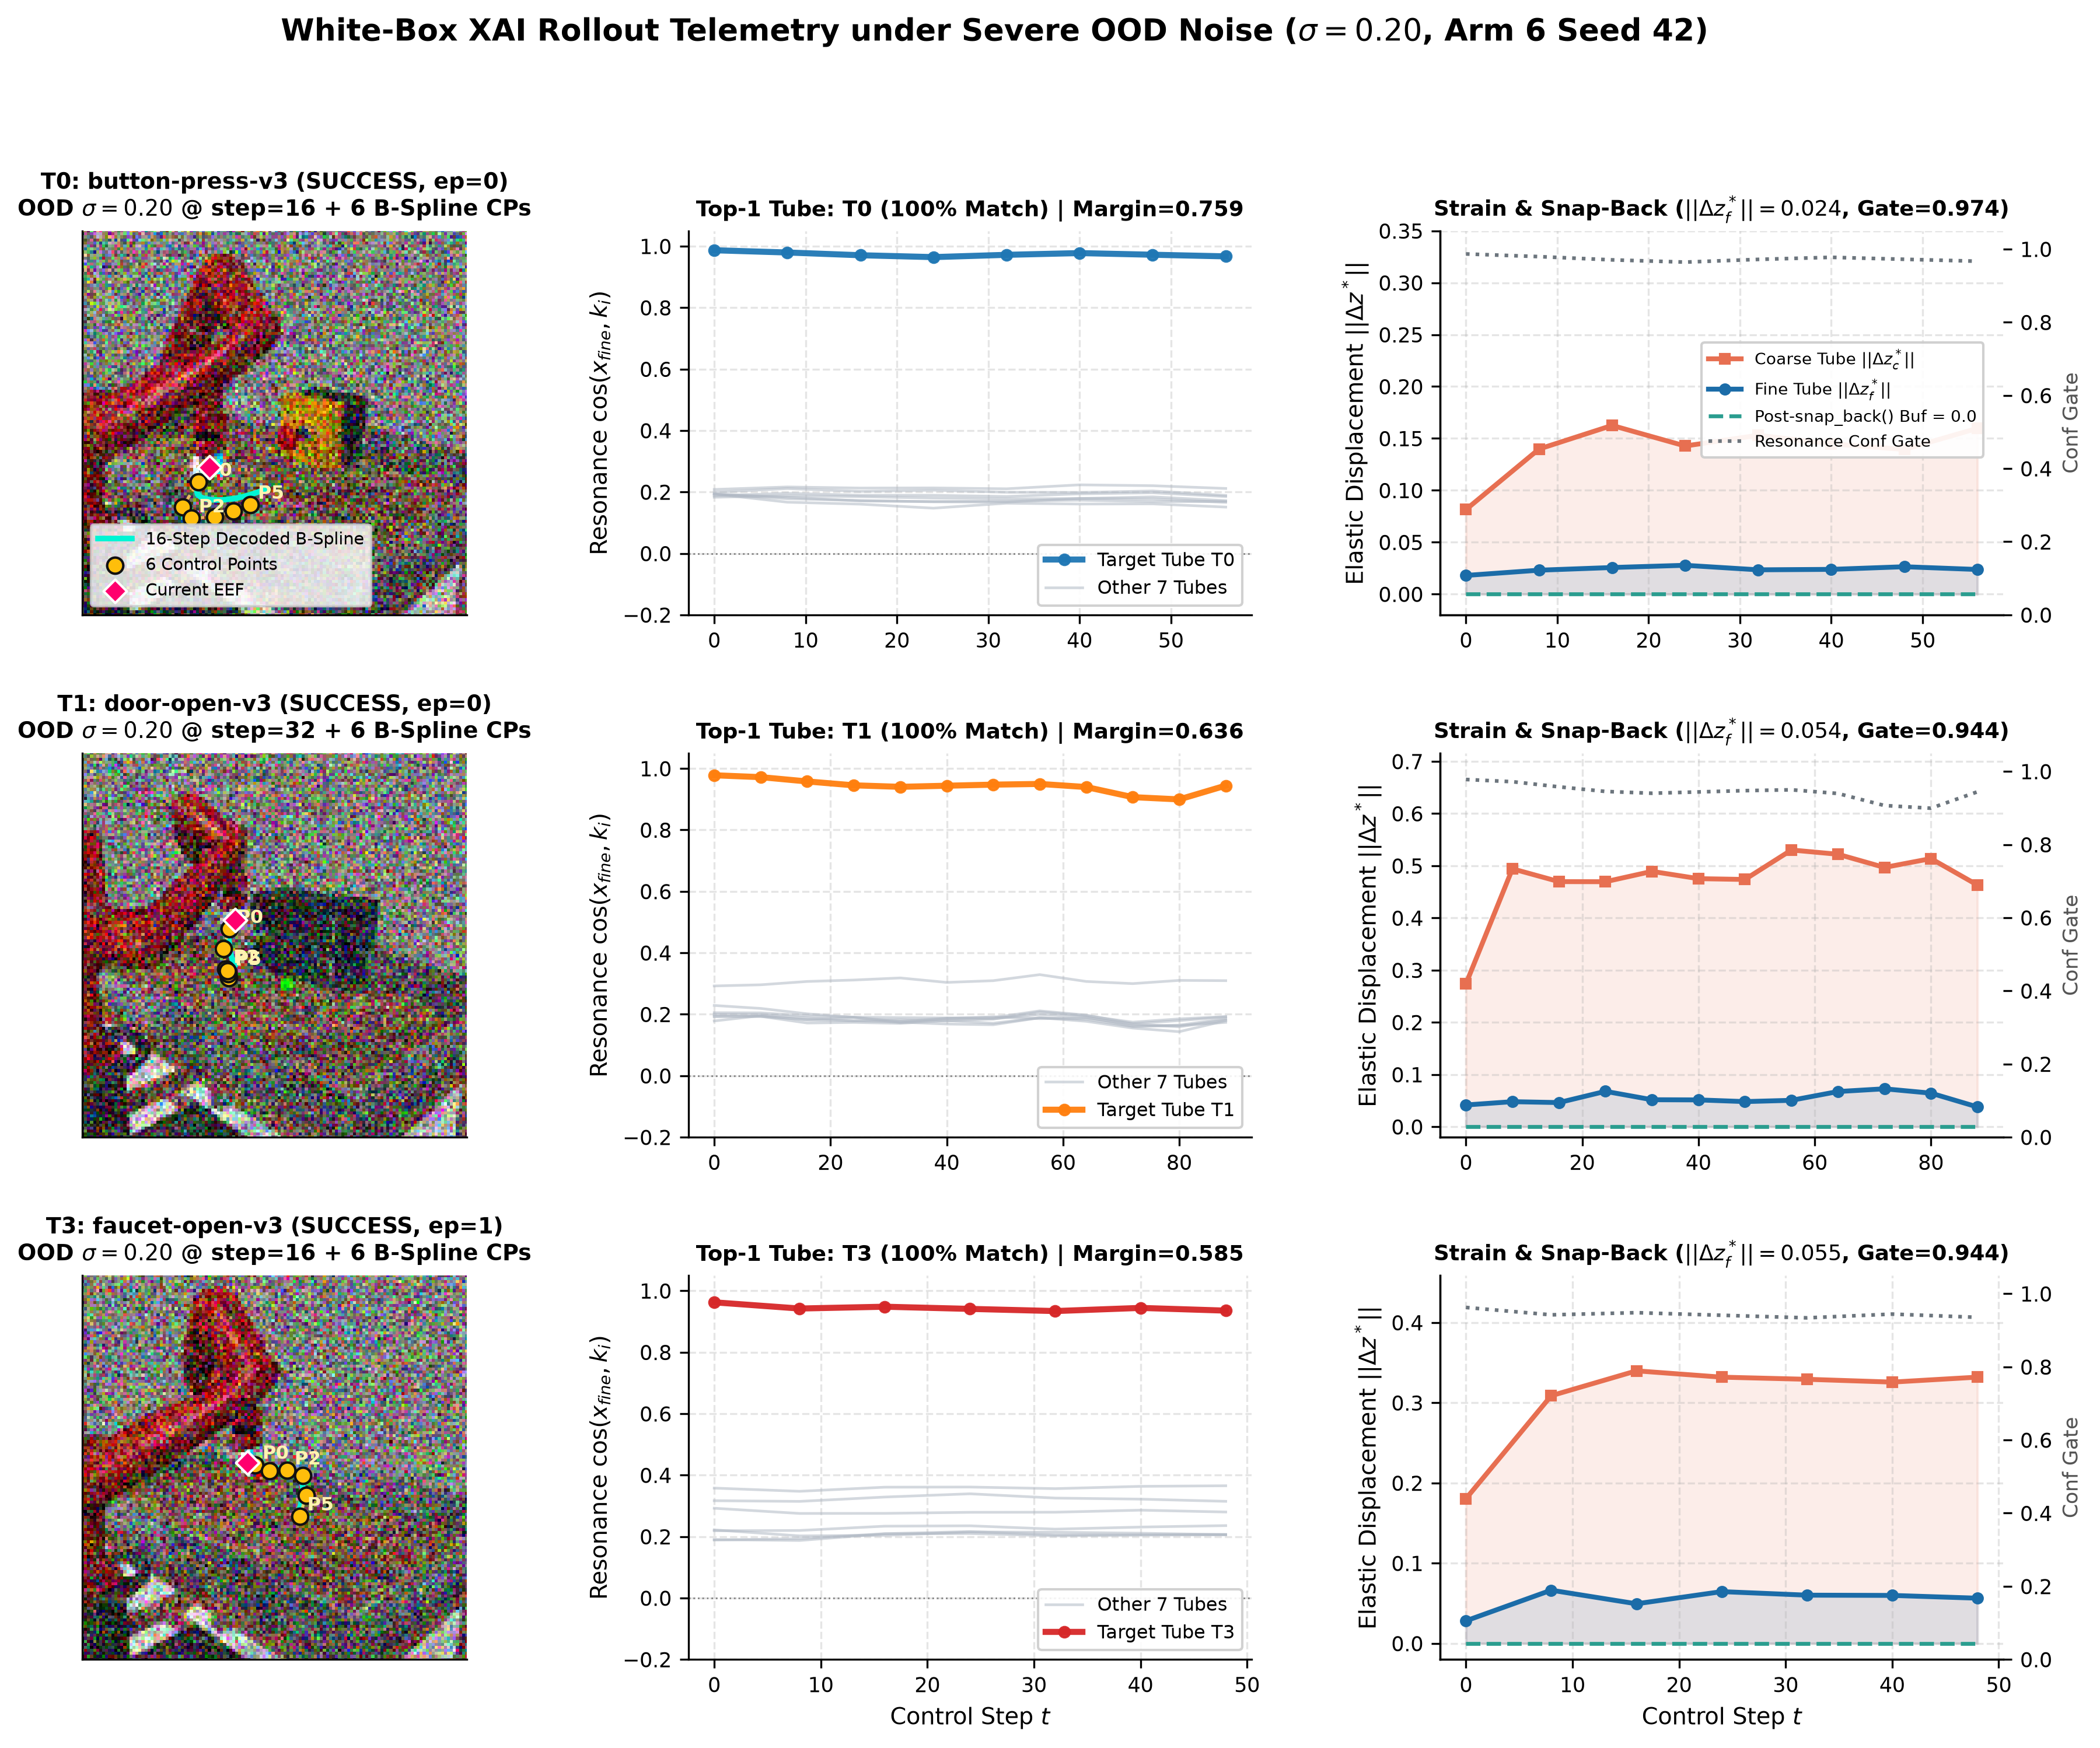
\includegraphics[width=0.84\textwidth]{../../outputs/figures/fig3_xai_telemetry_rollout.png}
  \caption{\textbf{Closed-Loop White-Box Rollout Telemetry \& B-Spline Safety Envelope.} Visualizes active ring selection confidence, $C^2$ cubic B-Spline knot trajectories, and bounded elastic displacement $\|\Delta\mathbf{z}^*\|_2$ resetting to $0.0000$ at episode boundaries.}
  \label{fig:xai_rollout}
\end{figure}

\subsection*{White-Box Surgical Fault Isolation \& Determinism Verification Protocol}
During closed-loop deployment, DTRA logs a structured per-tick inspection tuple comprising active \texttt{Cell ID}, matched \texttt{SharedBasisBank} slot ($b^* \in \{0,\dots,26\}$), Stage-2 CMC separation margin, active elastic compliance norm $\|\Delta\mathbf{z}^*\|_2$, and end-of-episode \texttt{post\_snap\_norm}. As Table~\ref{tab:callstack_log} verifies: (1)~early registrations (\texttt{T00}--\texttt{T49}) allocate foundational bases while later registrations (\texttt{T64}--\texttt{T99}) predominantly bind to existing primitives via \texttt{REUSE}; (2)~every newly registered slot maintains strict self-similarity $s_{kk} \ge 0.96$ while No-Encroachment projection actively reduces peak neighbor interference (e.g., \texttt{T79}: $0.8416 \to 0.7209$, \texttt{T99}: $0.9247 \to 0.8342$); and (3)~every trajectory terminates with exact $0.0000$ residual deformation, enabling surgical per-Cell quarantine or replacement without risking catastrophic cascade across prior motor skills.


\end{document}
% To monolithic models burning megawatts just to forget Task 0: How adorable.
